\documentclass[a4paper,14pt]{extarticle}
%\documentclass[a4paper]{article}
\usepackage[T2A]{fontenc}
\usepackage[utf8]{inputenc}
\usepackage[english,russian]{babel}
\usepackage{indentfirst}
\usepackage{amssymb}
\usepackage{amsfonts}
\usepackage{amsmath}
\usepackage{mathtext}
\usepackage{cite}
\usepackage{enumerate}
\usepackage{float}
\usepackage[top=1.5cm,bottom=1.5cm,left=2.5cm,right=1.5cm]{geometry}
\usepackage[unicode]{hyperref}
\usepackage{graphicx}
\usepackage{color}
\usepackage[colorinlistoftodos]{todonotes}
\usepackage[format=hang, labelsep=period, margin=8pt, figurename=Рис.]{caption}
\usepackage{listings}
\usepackage{subcaption}
%\usepackage{showkeys}
\usepackage[onehalfspacing, nodisplayskipstretch]{setspace}

\definecolor{dkgreen}{rgb}{0,0.6,0}
\definecolor{gray}{rgb}{0.5,0.5,0.5}
\definecolor{mauve}{rgb}{0.58,0,0.82}

\numberwithin{equation}{section}
\setcounter{secnumdepth}{3} % глубина нумеруемых разделов
\setcounter{tocdepth}{3} % глубина оглавления

\begin{document}
%\listoftodos
%\clearpage
\newpage
\begin{titlepage}
\newpage

\begin{center}
	Министерство образования и науки Российской Федерации \\
	%Федеральное государственное автономное образовательное учреждение \\ высшего профессионального образования \\
	<<МОСКОВСКИЙ ФИЗИКО-ТЕХНИЧЕСКИЙ ИНСТИТУТ>>\\(государственный университет)\\[0.5cm]
	ФАКУЛЬТЕТ ФИЗИЧЕСКОЙ И КВАНТОВОЙ ЭЛЕКТРОНИКИ\\
	КАФЕДРА ТВЕРДОТЕЛЬНОЙ ЭЛЕКТРОНИКИ И РАДИОФИЗИКИ\\
	%\hrulefill\\
\end{center}

\vspace{0.5em}

\begin{flushright}
На правах рукописи \\
УДК 519.63
\end{flushright}

\vspace{1em}

\begin{center}
	Новиков Алексей Викторович
\end{center}

\vspace{0.5em}

\begin{center}
	\textsc{\textbf{Численное моделирование\\ 
		волновых процессов в анизотропных твердых телах\\
		под действием ударной нагрузки}}\\[1cm]
	Выпускная квалификационная работа бакалавра\\
	Направление подготовки 010900\\
	«Прикладные математика и физика»\\
\end{center}

\vspace{2em}

\begin{flushleft}
	Заведующий кафедрой \hrulefill академик Гуляев Ю.В.\\[0.5cm]
	Научный руководитель \hrulefill к.ф.-м.н. Васюков А.В.\\[0.5cm]
	Студент-дипломник \hrulefill Новиков А.В.\\
\end{flushleft}

\vspace{\fill}
\begin{center}
Москва~--- 2014
\end{center}

\end{titlepage}

\setcounter{page}{2}
\tableofcontents
\clearpage
\newpage
\section*{Введение}
\addcontentsline{toc}{section}{Введение}
\setcounter{subsection}{0}
	
	В наши дни каждая отрасль промышленности имеет ряд специфических инженерных задач.
	Особое место среди них занимает подбор и исследование свойств конструкционных материалов, основы будущего продукта.
	За несколько последних десятилетий большое распространение получили полимерные композиционные материалы (ПКМ).
	
	Эти материалы, армируемые высокопрочными волокнами, приобретают ряд совершенно новых (по сравнению с металлами и сплавами) характеристик.
	Высокий модуль упругости и продел прочности в рассчёте на единицу массы, делают их весьма привлекательными для использования в авиационной и спортивной технике, автомобилестроении, судостроении, электронике и медицине.
	
	Сейчас можно увидеть как ПКМ все больше и больше вытесняют традиционные алюминиевые сплавы из авиастроения, позволяя создавать более лёгкие и прочные конструкции.
	Около этом 35-50\% деталей фюзеляжа современных военных и гражданских самолётов делается из ПКМ, армированных углеродными волокнами.
	Так, в аэробусе A-320 европейского гиганта Airbus ПКМ составляют 12,5\% массы самолёта.
	
	Применение композитов в авиации, создаёт потребность моделирования соударения композитной обшивки самолёта с другим телом.
	Эта задача относится к динамическим задачам механики деформируемого твёрдого тела (МДТТ).
	В данной работе исследуется распространение волн упругих деформаций в анизотропных твёрдых телах под действием ударной нагрузки.
	Целью работы является представить результаты некоторых численных расчётов картин деформаций слоистых анизотропных тел. 
	Для того чтобы понять особенности моделирования ПКМ необходимо сказать несколько слов об их структуре \cite{simamura}.
	
\subsection*{Структура композита}
	
	Обшивка самолёта обычно включает в себя несколько субпакетов композита, склеенных между собой эпоксидными смолами. 
	Основу каркаса представляют стрингеры, расположенные вдоль всей обшивки на некотором расстоянии друг от друга.
	Отдельно взятый субпакет состоит из одиннадцати монослоёв композита, спресованных в субпакет.
	Каждый мононслой -- это матрица из полимерных смол, армированная углеродными волокнами.
	Волокна укладываются вдоль одного выделенного напрвления, формируя вертикально-трансверсальную анизотропию в монослое.
	Монослои укладываются друг на друга под так, что углы между их выделенными направлениями составляют некоторую, вполне определённую, последовательность значений.
	Таким образом все выделенные направления лежат в плоскости субпакета и отличаются друг от друга поворотом вокруг оси укладки.
	
\subsection*{Численное моделирование}
		
	Волновые процессы, происходящие в таком многослойном материале, при соударении могут привести к возникновению областей разрушения, растрескивания материала.
	В виду существенной анизотропии материала, при таком нагружении конструкция может заметно терять прочность даже при отсутствии видимых повреждений.
	Поэтому расчёт деформаций в подобных конструкциях должен учитывыть полную волновую картину распространения, отражения и поглощения деформаций.
	
	В настоящее время наиболее широкое распространение для данного класса задач получил метод конечных элементов (МКЭ) \cite{jp}. 
	Однако МКЭ хорош для расчёта статических задач, и в ряде случаев не может обеспечить необходимые пространственные и временные разрешения с учётом влияния контактных границ в слоистых материалах.
	В этой связи, для решения системы уравнений МДТТ в данной работе применяется сеточно-характерестический численный метод, позволяющий преодолеть указанные трудности \cite{magomedov, petrov_book, petrov_tormasov_holodov, petrov}.
	
\subsection*{Обзор литературы}
	
	Исчерпывающую информацию о физике деформаций, происходящих в твёрдом теле можно вынести из фундаментальных книг по МДТТ \cite{rabotnov,novatsky,sedov}.
	Теория пластичности описана в \cite{ilyushin}.
	Теория упругости для анизотропных тел подробно разобрана в \cite{lehnitsky}.
	Механика деформаций применительно к композиционным материалам описана в \cite{resler,pobedrya,bazhenov,simamura}.
	Там же содержатся основные сведения о механике анизотропных тел.
	
	Математическая модель МДТТ в самом общем виде представляет собой гиперболическую систему квазилинейных уравнений в частных производных.
	Описание квазилинейных систем можно найти в \cite{rozhdestvenskiy}. Математические аспекты численного решения гиперболических систем изложены в \cite{kulikovskiy}.
	
	Подробное и последовательное изложении теории численных методов и её приложений есть в \cite{petrov_book}.
	Решению систем гиперболических уравнений сеточно-характеристическим методом посвящена книга \cite{magomedov}.
	Численное моделирование механики сплошных сред излагается в \cite{belocerkovsky,kukudzhanov_main}.
	Стоит отдельно отметить книгу \cite{kukudzhanov_main}, в которой лаконично описаны как и физика сплошных сред, так и численные методы, использемые в механике сплошных сред.
	Основной акцент автор сделал на моделировании больших деформаций и разрушения материалов, что оказалось безмерно полезно при создании этой работы.
	В работе \cite{petrov_tormasov_holodov} исследуется прохождение импульса сжатия через различные многослойные конструкции в одномерной и двумерной постановке для упругого и упругоидеальнопластического материала. Описаны эффекты кумуляции вторичных волн и сепарации.
	В \cite{ivanov_kondaurov_petrov_holodov} сформулирована математическая модель упруговязкопластической повреждающейся среды, учитывающая конечные деформации материала. 
	Для рассчётов испульзуется гибридная схема.
	Такие схемы, позвяющие считать разрывные решения с первым порядком точности, а гладкие со вторым, описаны в \cite{fedorenko}.
	Статья \cite{kukudzhanov1} посвящена изучению распространения одномерных упругопластических волн с учётом влияния скорости деформации. 
	Скорость деформаций существенно влияет на уравнения состояния твёрдых тел, особенно металлов и различных полимеров.
	Полноценная модель упруго-вязко-пластической среды в многомерном случае описана в \cite{kukudzhanov2}. 
	Для построения решения используются характеристические поверхности. Доказана устойчивость, рассмотрены преимущества в сравнении с упруго-пластической моделью.
	
	
	Основными работы, посвящёнными разработке численных методов и пакетов программ моделирования МДТТ в случае трёх пространственных переменных с явным выделением контакта, послужвишими фундаментом создания этой, являются \cite{a4,a6}.
	В \cite{a6} описывается численное решение уравнений МДТТ в трёхмерной постановке сеточно-характеристическим методом на тетраэдрических неструктурированных сетках.
	В \cite{a4} обсуждаются технические аспекты разработки параллельной версии сеточно-характерестического метода. 
	Статья \cite{favorskaya} посвящена численному моделированию линейно упругого анизотропного тела с применением сеточно-характеристического метода.
	

\clearpage
\newpage
\section*{Глава 1\\Основные уравнения механики деформируемого твёрдого тела}
\addcontentsline{toc}{section}{Глава 1. Основные уравнения механики деформируемого твёрдого тела}
\setcounter{section}{1}
\setcounter{subsection}{0}
\setcounter{equation}{0}

\subsection{Уравнения механики деформируемого твёрдого тела}
	
	Основные определяющие соотношения МДТТ включают в себя уравнения движения и реологические соотношения \cite{novatsky,sedov,rabotnov}.
	Посление определяют сопротивление материала по отношению к внешнему воздействию.
\begin{align}
	\label{initial_equations}
	\rho\dot{v}_i &= \nabla_j\sigma_{ij}+f_i & \textrm{(уравнения движения)}\nonumber\\
	\dot{\sigma}_{ij} &= q_{ijkl}\dot{\varepsilon}_{kl}+F_{ij} & \textrm{(реологические соотношения).}
\end{align}
	Здесь $\rho$ – плотность среды, $v_i$ – компоненты скорости смещения,
	$\sigma_{ij}$, $\varepsilon_{ij}$ -- компоненты тензоров напряжений и деформаций,
	$\nabla_j$ – ковариантная производная по $j$-й координате, $f_i$ – массовые
	силы, действующие на единицу объёма, $F_{ij}$ -- правая часть, используемая, например, для описания диссипации в моделях с учётом вязкости.

	В случае малых деформаций тензор скоростей деформаций $e_{ij}=\dot{\varepsilon}_{ij}$ 
	выражается через компоненты скорости смещения линейным образом \cite{landau_lifshits}:
	
\begin{equation}
	\label{small_deformation}
	e_{ij}=\frac{1}{2}(\nabla_j v_i+\nabla_i v_j).
\end{equation}

	Вид компонент тензора 4-го порядка $q_{ijkl}$ и правой части $F_{ij}$ определяется реологией среды.

	Для замыкания системы уравнений \eqref{initial_equations} её необходимо дополнить уравнением состояния, определяющим зависимость плотности от напряжений:

\begin{equation}
	\rho=\rho_0e^{\frac{p}{K}},
\end{equation}
	где $p=-\frac{1}{3}\sum\sigma_{kk}$ -- давление, $K=\lambda+\frac{2}{3}\mu$ -- коэффициент всестороннего сжатия, $\lambda$ и $\mu$ -- параметры Ламе.

	Параметры Ламе зависят от материала и связаны с модулем продольной упругости и коэффициентом Пуассона следующим образом:
\begin{align}
	\label{lame_parameters}
	\lambda &= \frac{E\nu}{(1+\nu)(1-2\nu)}
	\nonumber\\
	\mu &= G=\frac{E}{2(1+\nu)}.
\end{align}
	Здесь $E$ -- модуль продольной упругости, $\nu$ -- коэффициент Пуассона, $G$ -- модуль сдвига.
\clearpage
\newpage

\subsection{Приближение линейно упругого тела}
	
	В простейшем случае линейной упругости тензор $q_{ijkl}$ и правая часть $F_{ij}$ в \eqref{initial_equations} принимают следующий вид \cite{landau_lifshits}:
\begin{align}
	\label{tensor_qijkl_elastic}
	q_{ijkl}&=\lambda\delta_{ij}\delta_{kl}+\mu(\delta_{ik}\delta_{jl}+\delta_{il}
	\delta_{jk}),\nonumber\\
	F_{ij}&=0.
\end{align}
	В этом соотношении $\lambda$ и $\mu$ -- параметры Ламе, $\delta_{ij}$ -- символ Кронекера.
	
	Уравнения \eqref{initial_equations} в приближении \eqref{small_deformation} будут выглядеть следующим образом: 
\begin{align}
	\label{simple_equations}
	\frac{\partial{v_x}}{\partial{t}}&=\frac{1}{\rho}(\frac{\partial{\sigma_{xx}}}{\partial{x}}+\frac{\partial{\sigma_{xy}}}{\partial{y}}+\frac{\partial{\sigma_{xz}}}{\partial{z}})
	\nonumber\\
	\frac{\partial{v_y}}{\partial{t}}&=\frac{1}{\rho}(\frac{\partial{\sigma_{xy}}}{\partial{x}}+\frac{\partial{\sigma_{yy}}}{\partial{y}}+\frac{\partial{\sigma_{yz}}}{\partial{z}})
	\nonumber\\
	\frac{\partial{v_z}}{\partial{t}}&=\frac{1}{\rho}(\frac{\partial{\sigma_{xz}}}{\partial{x}}+\frac{\partial{\sigma_{yz}}}{\partial{y}}+\frac{\partial{\sigma_{zz}}}{\partial{z}})
	\nonumber\\
	\frac{\partial{\sigma_{xx}}}{\partial{t}}&=(\lambda+2\mu)\frac{\partial{v_x}}{\partial{x}}+\lambda\frac{\partial{v_y}}{\partial{y}}+\lambda\frac{\partial{v_z}}{\partial{z}}
	\nonumber\\
	\frac{\partial{\sigma_{xy}}}{\partial{t}}&=\mu(\frac{\partial{v_x}}{\partial{y}}+\frac{\partial{v_y}}{\partial{x}})
	\nonumber\\
	\frac{\partial{\sigma_{xz}}}{\partial{t}}&=\mu(\frac{\partial{v_x}}{\partial{z}}+\frac{\partial{v_z}}{\partial{x}})
	\nonumber\\
	\frac{\partial{\sigma_{yy}}}{\partial{t}}&=\lambda\frac{\partial{v_x}}{\partial{x}}+(\lambda+2\mu)\frac{\partial{v_y}}{\partial{y}}+\lambda\frac{\partial{v_z}}{\partial{z}}
	\nonumber\\
	\frac{\partial{\sigma_{yz}}}{\partial{t}}&=\mu(\frac{\partial{v_z}}{\partial{y}}+\frac{\partial{v_y}}{\partial{z}})
	\nonumber\\
	\frac{\partial{\sigma_{zz}}}{\partial{t}}&=\lambda\frac{\partial{v_x}}{\partial{x}}+\lambda\frac{\partial{v_y}}{\partial{y}}+(\lambda+2\mu)\frac{\partial{v_z}}{\partial{z}}
\end{align}

	Обозначив искомый вектор $\vec{u}=\{v_x,v_y,v_z,\sigma_{xx},\sigma_{xy},\sigma_{xz},\sigma_{yy},\sigma_{yz},\sigma_{zz}\}^T$, уравнения \eqref{simple_equations} можно переписать в матричной форме:

\begin{equation}
	\label{simple_matrix_equation}
	\frac{\partial\vec{u}}{\partial{t}}+\mathbf{A}_x\frac{\partial\vec{u}}{\partial{x}}+
	\mathbf{A}_y\frac{\partial\vec{u}}{\partial{y}}+
	\mathbf{A}_z\frac{\partial\vec{u}}{\partial{z}}=0.
\end{equation}

	Для линейно упругого тела матрицы $\mathbf{A}_x$, $\mathbf{A}_y$, $\mathbf{A}_z$ в \eqref{simple_matrix_equation} принимают следующий вид.

\begin{align}
\label{isotropic_mat1}
\mathbf{A}_x =
\left( \begin{array}{cccccccccccc}
0 & 0 & 0 & -\frac 1 \rho & 0 & 0 & 0 & 0 & 0 \\ 
0 & 0 & 0 & 0 & -\frac 1 \rho & 0 & 0 & 0 & 0 \\ 
0 & 0 & 0 & 0 & 0 & -\frac 1 \rho & 0 & 0 & 0 \\ 
-(\lambda+2\mu) & 0 & 0 & 0 & 0 & 0 & 0 & 0 & 0 \\ 
0 & -\mu & 0 & 0 & 0 & 0 & 0 & 0 & 0 \\ 
0 & 0 & -\mu & 0 & 0 & 0 & 0 & 0 & 0 \\ 
-\lambda & 0 & 0 & 0 & 0 & 0 & 0 & 0 & 0 \\ 
0 & 0 & 0 & 0 & 0 & 0 & 0 & 0 & 0 \\ 
-\lambda & 0 & 0 & 0 & 0 & 0 & 0 & 0 & 0  
\end{array} \right),
\end{align} 
\begin{align}
\label{isotropic_mat2}
\mathbf{A}_y =
\left( \begin{array}{cccccccccccc}
0 & 0 & 0 & 0 & -\frac 1 \rho & 0 & 0 & 0 & 0 \\ 
0 & 0 & 0 & 0 & 0 & 0 & -\frac 1 \rho & 0 & 0 \\ 
0 & 0 & 0 & 0 & 0 & 0 & 0 & -\frac 1 \rho & 0 \\ 
0 & -\lambda & 0 & 0 & 0 & 0 & 0 & 0 & 0 \\ 
-\mu & 0 & 0 & 0 & 0 & 0 & 0 & 0 & 0 \\ 
0 & 0 & 0 & 0 & 0 & 0 & 0 & 0 & 0 \\ 
0 & -(\lambda+2\mu) & 0 & 0 & 0 & 0 & 0 & 0 & 0 \\ 
0 & 0 & -\mu & 0 & 0 & 0 & 0 & 0 & 0 \\ 
0 & -\lambda & 0 & 0 & 0 & 0 & 0 & 0 & 0  
\end{array} \right),
\end{align}
\begin{align}
\label{isotropic_mat3}
\mathbf{A}_z =
\left( \begin{array}{cccccccccccc}
0 & 0 & 0 & 0 & 0 & -\frac 1 \rho & 0 & 0 & 0 \\ 
0 & 0 & 0 & 0 & 0 & 0 & 0 & -\frac 1 \rho & 0 \\ 
0 & 0 & 0 & 0 & 0 & 0 & 0 & 0 & -\frac 1 \rho \\ 
0 & 0 & -\lambda & 0 & 0 & 0 & 0 & 0 & 0 \\ 
0 & 0 & 0 & 0 & 0 & 0 & 0 & 0 & 0 \\ 
-\mu & 0 & 0 & 0 & 0 & 0 & 0 & 0 & 0 \\ 
0 & 0 & -\lambda & 0 & 0 & 0 & 0 & 0 & 0 \\ 
0 & -\mu & 0 & 0 & 0 & 0 & 0 & 0 & 0 \\ 
0 & 0 & -(\lambda+2\mu) & 0 & 0 & 0 & 0 & 0 & 0  
\end{array} \right).
\end{align}\\
	Аналогично можно записать более общую систему \eqref{initial_equations} в виде:

\begin{equation}
	\label{matrix_equation}
	\frac{\partial\vec{u}}{\partial{t}}+\mathbf{A}_x\frac{\partial\vec{u}}{\partial{x}}+
	\mathbf{A}_y\frac{\partial\vec{u}}{\partial{y}}+
	\mathbf{A}_z\frac{\partial\vec{u}}{\partial{z}}=\vec{f}.
\end{equation}
	Здесь $\vec{f}$ -- вектор правых частей, размерность которого равна размерности исходной системы, а выражения для компонентов зависят от реологии среды.
	Точный вид матриц $\mathbf{A}_x$, $\mathbf{A}_y$, $\mathbf{A}_z$ зависит от реологии среды.
	
	Система, записанная в общем виде \eqref{matrix_equation}, представляет из себя \textit{систему квазилинейных уравнений} в частных производных\cite{rozhdestvenskiy}, где $\mathbf{A}_x = \mathbf{A}_x(t, x, y, z, \vec{u})$, $\mathbf{A}_y = \mathbf{A}_y(t, x, y, z, \vec{u})$, $\mathbf{A}_z = \mathbf{A}_z(t, x, y, z, \vec{u})$, $\vec{f} = \vec{f}(t, x, y, z, \vec{u})$ в общем случае.
	Она будет линейной в случае: $\mathbf{A}_x = \mathbf{A}_x(t, x, y, z)$, $\mathbf{A}_y = \mathbf{A}_y(t, x, y, z)$, $\mathbf{A}_z = \mathbf{A}_z(t, x, y, z)$.
	
	Для широкого класса задач МДТТ система уравнений \eqref{matrix_equation} имеет \textit{гиперболический} тип. Это значит, что существуют несколько интегралов движения и система может быть решена методом характеристик.
\clearpage
\newpage

\subsection{Линейно-упругое приближение анизотропного тела}

	Математическая модель анизотропной среды для трехмерного случая описывается системой уравнений\cite{favorskaya}:
\begin{small}
\begin{align}
	\label{anisotropic_equations}
	\frac{\partial{v_x}}{\partial{t}}&=\frac{1}{\rho}(\frac{\partial{\sigma_{xx}}}{\partial{x}}+\frac{\partial{\sigma_{xy}}}{\partial{y}}+\frac{\partial{\sigma_{xz}}}{\partial{z}})
	\nonumber\\
	\frac{\partial{v_y}}{\partial{t}}&=\frac{1}{\rho}(\frac{\partial{\sigma_{xy}}}{\partial{x}}+\frac{\partial{\sigma_{yy}}}{\partial{y}}+\frac{\partial{\sigma_{yz}}}{\partial{z}})
	\nonumber\\
	\frac{\partial{v_z}}{\partial{t}}&=\frac{1}{\rho}(\frac{\partial{\sigma_{xz}}}{\partial{x}}+\frac{\partial{\sigma_{yz}}}{\partial{y}}+\frac{\partial{\sigma_{zz}}}{\partial{z}})
	\nonumber\\
	\frac{\partial{\sigma_{xx}}}{\partial{t}}&=c_{11}\frac{\partial{v_x}}{\partial{x}}+c_{12}\frac{\partial{v_y}}{\partial{y}}+c_{13}\frac{\partial{v_z}}{\partial{z}}+c_{14}(\frac{\partial{v_z}}{\partial{y}}+\frac{\partial{v_y}}{\partial{z}})+c_{15}(\frac{\partial{v_z}}{\partial{x}}+\frac{\partial{v_x}}{\partial{z}})+c_{16}(\frac{\partial{v_y}}{\partial{x}}+\frac{\partial{v_x}}{\partial{y}})
	\nonumber\\
	\frac{\partial{\sigma_{yy}}}{\partial{t}}&=c_{12}\frac{\partial{v_x}}{\partial{x}}+c_{22}\frac{\partial{v_y}}{\partial{y}}+c_{23}\frac{\partial{v_z}}{\partial{z}}+c_{24}(\frac{\partial{v_z}}{\partial{y}}+\frac{\partial{v_y}}{\partial{z}})+c_{25}(\frac{\partial{v_z}}{\partial{x}}+\frac{\partial{v_x}}{\partial{z}})+c_{26}(\frac{\partial{v_y}}{\partial{x}}+\frac{\partial{v_x}}{\partial{y}})
	\nonumber\\
	\frac{\partial{\sigma_{zz}}}{\partial{t}}&=c_{13}\frac{\partial{v_x}}{\partial{x}}+c_{23}\frac{\partial{v_y}}{\partial{y}}+c_{33}\frac{\partial{v_z}}{\partial{z}}+c_{34}(\frac{\partial{v_z}}{\partial{y}}+\frac{\partial{v_y}}{\partial{z}})+c_{35}(\frac{\partial{v_z}}{\partial{x}}+\frac{\partial{v_x}}{\partial{z}})+c_{36}(\frac{\partial{v_y}}{\partial{x}}+\frac{\partial{v_x}}{\partial{y}})
	\nonumber\\
	\frac{\partial{\sigma_{yz}}}{\partial{t}}&=c_{14}\frac{\partial{v_x}}{\partial{x}}+c_{24}\frac{\partial{v_y}}{\partial{y}}+c_{34}\frac{\partial{v_z}}{\partial{z}}+c_{44}(\frac{\partial{v_z}}{\partial{y}}+\frac{\partial{v_y}}{\partial{z}})+c_{45}(\frac{\partial{v_z}}{\partial{x}}+\frac{\partial{v_x}}{\partial{z}})+c_{46}(\frac{\partial{v_y}}{\partial{x}}+\frac{\partial{v_x}}{\partial{y}})
	\nonumber\\
	\frac{\partial{\sigma_{xz}}}{\partial{t}}&=c_{15}\frac{\partial{v_x}}{\partial{x}}+c_{25}\frac{\partial{v_y}}{\partial{y}}+c_{35}\frac{\partial{v_z}}{\partial{z}}+c_{45}(\frac{\partial{v_z}}{\partial{y}}+\frac{\partial{v_y}}{\partial{z}})+c_{55}(\frac{\partial{v_z}}{\partial{x}}+\frac{\partial{v_x}}{\partial{z}})+c_{56}(\frac{\partial{v_y}}{\partial{x}}+\frac{\partial{v_x}}{\partial{y}})
	\nonumber\\
	\frac{\partial{\sigma_{xy}}}{\partial{t}}&=c_{16}\frac{\partial{v_x}}{\partial{x}}+c_{26}\frac{\partial{v_y}}{\partial{y}}+c_{36}\frac{\partial{v_z}}{\partial{z}}+c_{46}(\frac{\partial{v_z}}{\partial{y}}+\frac{\partial{v_y}}{\partial{z}})+c_{56}(\frac{\partial{v_z}}{\partial{x}}+\frac{\partial{v_x}}{\partial{z}})+c_{66}(\frac{\partial{v_y}}{\partial{x}}+\frac{\partial{v_x}}{\partial{y}})
\end{align}
\end{small}
	
	Коээфициенты в последних шести уравнениях - составляющие \textit{тензора упругих постоянных} четвёртого ранга, который в данном случае записывается в виде матрицы:

\begin{align}
\label{anisotropic_tensor}	
c_{ik} =
\left( \begin{array}{cccccccccccc}
c_{11} & c_{12} & c_{13} & c_{14} & c_{15} & c_{16} \\ 
c_{12} & c_{22} & c_{23} & c_{24} & c_{25} & c_{26} \\ 
c_{13} & c_{23} & c_{33} & c_{34} & c_{35} & c_{36} \\ 
c_{14} & c_{24} & c_{34} & c_{44} & c_{45} & c_{46} \\ 
c_{15} & c_{25} & c_{35} & c_{45} & c_{55} & c_{56} \\ 
c_{16} & c_{26} & c_{36} & c_{46} & c_{56} & c_{66}
\end{array} \right).
\end{align}\\
	
	Собрав производные вдоль различных осей по матрицам $\mathbf{A}_x$, $\mathbf{A}_y$, $\mathbf{A}_z$ и снова обозначив искомый вектор $\vec{u}=\{v_x,v_y,v_z,\sigma_{xx},\sigma_{xy},\sigma_{xz},\sigma_{yy},\sigma_{yz},\sigma_{zz}\}^T$, уравнения \eqref{anisotropic_equations} предстанут в виде \eqref{simple_matrix_equation} с соответствующими матрицами:
	
\begin{align}
\label{anisotropic_mat1}	
\mathbf{A}_x = - 
\left( \begin{array}{cccccccccccc}
0 & 0 & 0 & \frac 1 \rho & 0 & 0 & 0 & 0 & 0 \\ 
0 & 0 & 0 & 0 & \frac 1 \rho & 0 & 0 & 0 & 0 \\ 
0 & 0 & 0 & 0 & 0 & \frac 1 \rho & 0 & 0 & 0 \\ 
c_{11} & c_{16} & c_{15} & 0 & 0 & 0 & 0 & 0 & 0 \\ 
c_{16} & c_{66} & c_{56} & 0 & 0 & 0 & 0 & 0 & 0 \\
c_{15} & c_{56} & c_{55} & 0 & 0 & 0 & 0 & 0 & 0 \\ 
c_{12} & c_{26} & c_{25} & 0 & 0 & 0 & 0 & 0 & 0 \\ 
c_{14} & c_{46} & c_{45} & 0 & 0 & 0 & 0 & 0 & 0 \\ 
c_{13} & c_{36} & c_{35} & 0 & 0 & 0 & 0 & 0 & 0
\end{array} \right),
\end{align} 
\begin{align}
\label{anisotropic_mat2}
\mathbf{A}_y = - 
\left( \begin{array}{cccccccccccc}
0 & 0 & 0 & 0 & \frac 1 \rho & 0 & 0 & 0 & 0 \\ 
0 & 0 & 0 & 0 & 0 & 0 & \frac 1 \rho & 0 & 0 \\ 
0 & 0 & 0 & 0 & 0 & 0 & 0 & \frac 1 \rho & 0 \\ 
c_{16} & c_{12} & c_{14} & 0 & 0 & 0 & 0 & 0 & 0 \\ 
c_{66} & c_{26} & c_{46} & 0 & 0 & 0 & 0 & 0 & 0 \\
c_{56} & c_{25} & c_{45} & 0 & 0 & 0 & 0 & 0 & 0 \\
c_{26} & c_{22} & c_{24} & 0 & 0 & 0 & 0 & 0 & 0 \\ 
c_{46} & c_{24} & c_{44} & 0 & 0 & 0 & 0 & 0 & 0 \\
c_{36} & c_{23} & c_{34} & 0 & 0 & 0 & 0 & 0 & 0   
\end{array} \right),
\end{align}
\begin{align}
\label{anisotropic_mat3}
\mathbf{A}_z = - 
\left( \begin{array}{cccccccccccc}
0 & 0 & 0 & 0 & 0 & \frac 1 \rho & 0 & 0 & 0 \\ 
0 & 0 & 0 & 0 & 0 & 0 & 0 & \frac 1 \rho & 0 \\ 
0 & 0 & 0 & 0 & 0 & 0 & 0 & 0 & \frac 1 \rho \\ 
c_{15} & c_{14} & c_{13} & 0 & 0 & 0 & 0 & 0 & 0 \\ 
c_{56} & c_{46} & c_{36} & 0 & 0 & 0 & 0 & 0 & 0 \\
c_{55} & c_{45} & c_{35} & 0 & 0 & 0 & 0 & 0 & 0 \\ 
c_{25} & c_{24} & c_{23} & 0 & 0 & 0 & 0 & 0 & 0 \\ 
c_{45} & c_{44} & c_{34} & 0 & 0 & 0 & 0 & 0 & 0 \\ 
c_{35} & c_{34} & c_{33} & 0 & 0 & 0 & 0 & 0 & 0  
\end{array} \right).
\end{align}\\

	Подробнее, общий случай анизотропного упругого тела и различные типы анизотропии будут рассмотрены в Главе 2.

\clearpage
\newpage
\section*{Глава 2\\Основные соотношения механики упругих анизотропных тел}
\addcontentsline{toc}{section}{Глава 2. Основные соотношения механики упругих анизотропных тел}
\setcounter{section}{2}
\setcounter{subsection}{0}
\setcounter{equation}{0}

\subsection{Тензор упругих постоянных}

	В одномерном случае при не слишком больших деформациях напряжение будет линейно зависеть от деформаций.
	В случае трёх пространственных переменных эта связь в самом общем случае будет иметь вид\cite{resler}:
\begin{align}
	\label{rheology_equation}
	\sigma_{ij} &= C_{ijkl}\varepsilon_{kl},
\end{align}
	где $\sigma_{ij}$ -- тензор напряжений, $\varepsilon_{kl}$ -- тензор деформаций, $C_{ijkl}$ -- тензор упругих постоянных. 
	Это уравнение, по сути, реологическое соотношение из \eqref{initial_equations}.
	
	В общем случае $C_{ijkl}$ имеет $3^{4} = 81$ компоненты. Однако, тензор деформаций симметричен по определению и имеет шесть независимых компонент.
	Тензор напряжений также симметричен, поскольку при его определении мы не учитываем изгибающие моменты\cite{resler}. 
	Во всяком случае, существенно то, что тензор напряжений может быть приведён в симметричному виду\cite{landau_lifshits}.
	
	Таким образом количество независимых компонент тензора упругих постоянных сокращается до $6^{2} = 36$.
	Далее, в упругом случае, тензор упругих постоянных обладает дополнительной симметрией, за счёт потенциальности упругого деформирования. Обозначим $w$ -- потенциал уругости, тогда по определению: $dw = \sigma_{ij} d\varepsilon_{ij}$.
	Учитывая, что: 
\begin{align}
	C_{ijkl} &= \frac{\partial{\sigma_{ij}}}{\partial{\varepsilon_{kl}}},
\end{align}
	имеем:
\begin{align}
	C_{ijkl} &= \frac{\partial^{2}{w}}{\partial{\varepsilon_{ij}\varepsilon_{kl}}}.
\end{align}
	Последовательность вычисления производных в данном случае не имеет значения, поэтому $C_{ijkl} = C_{klij}$ и тензор упругих постоянных имеет 21 независимую компоненту.
	Выражение \eqref{rheology_equation} с симметричной матрицей упругих постоянных \eqref{anisotropic_tensor} теперь удобно записать в виде:
\begin{align}
\left( \begin{array}{cccccccccccc}
\sigma_{11} \\
\sigma_{22} \\
\sigma_{33} \\
\sigma_{23} \\
\sigma_{13} \\
\sigma_{12} 
\end{array} \right){}
= \left( \begin{array}{cccccccccccc}
c_{11} & c_{12} & c_{13} & c_{14} & c_{15} & c_{16} \\ 
c_{12} & c_{22} & c_{23} & c_{24} & c_{25} & c_{26} \\ 
c_{13} & c_{23} & c_{33} & c_{34} & c_{35} & c_{36} \\ 
c_{14} & c_{24} & c_{34} & c_{44} & c_{45} & c_{46} \\ 
c_{15} & c_{25} & c_{35} & c_{45} & c_{55} & c_{56} \\ 
c_{16} & c_{26} & c_{36} & c_{46} & c_{56} & c_{66}
\end{array} \right){}
\left( \begin{array}{cccccccccccc}
\varepsilon_{11} \\
\varepsilon_{22} \\
\varepsilon_{33} \\
\varepsilon_{23} \\
\varepsilon_{13} \\
\varepsilon_{12}
\end{array} \right)
\end{align}

\subsection{Исследование общего случая}

Теперь перейдём к исследованию общего случая.
Как уже было сказано, обозначив $\vec{u}=\{v_x,v_y,v_z,\sigma_{xx},\sigma_{xy},\sigma_{xz},\sigma_{yy},\sigma_{yz},\sigma_{zz}\}^T$ -- вектор искомых решений, уравнения \eqref{anisotropic_equations} предстанут в виде:

\begin{equation}
	\label{matrix_anisotropy_equation}
	\frac{\partial\vec{u}}{\partial{t}}+\mathbf{A}_x\frac{\partial\vec{u}}{\partial{x}}+
	\mathbf{A}_y\frac{\partial\vec{u}}{\partial{y}}+
	\mathbf{A}_z\frac{\partial\vec{u}}{\partial{z}}=0,
\end{equation}
	где $\mathbf{A}_x$, $\mathbf{A}_y$, $\mathbf{A}_z$ -- матрицы \eqref{anisotropic_mat1}, \eqref{anisotropic_mat2}, \eqref{anisotropic_mat3} соответственно, из пункта 1.3.
	
	Для применения сеточно-характеристического метода будет необходимо будет разделить систему на девять уравнений -- перейти к \textit{инвариантам Римана}.
	Для это необходимо будет диагонализовать матрицы $\mathbf{A}_x$, $\mathbf{A}_y$, $\mathbf{A}_z$.
	Ввиду их блочной структуры представляется возможным сделать это аналитически\cite{favorskaya}.
	
	Итак, обозначая  $\lambda^{2} = t$, где $\lambda$ -- собственные значения матрицы $\mathbf{A}_x$, а $t$ задаются кубическим уравнением:
\begin{small}
\begin{align}	
	\label{eigenvalue_equation1}
	t^{3} &- \frac{1}{\rho}(c_{11} + c_{55} + c_{66})\;t^{2} - \frac{1}{\rho^{2}}(c_{15}^{2} - c_{11}c_{55} + c_{16}^{2} - c_{11}c_{66} + c_{56}^{2} - c_{55}c_{66})\;t\;+ \nonumber\\
	&+ \frac{1}{\rho^{3}}((c_{56}^{2} - c_{55}c_{66})c_{11} + (c_{16}c_{55} - c_{15}c_{56})c_{16} + (c_{15}c_{66} - c_{16}c_{56})c_{15}) = 0,
\end{align}
\end{small}
	решения которого могут быть аналитически вычисленны с помощью тригонометрической формулы Виета. В итоге, имеем следующие собственные значения $\mathbf{A}_x$:
\begin{align}
	\left\{\sqrt{t_{11}},\;-\sqrt{t_{11}},\;\sqrt{t_{12}},\;-\sqrt{t_{12}},\;\sqrt{t_{13}},\;-\sqrt{t_{13}},\;0,\;0,\;0\right\},
\end{align}
	где $t_{11}$, $t_{12}$, $t_{13}$ -- действительные положительные корни \eqref{eigenvalue_equation1}.
	
	Аналогично для $\mathbf{A}_y$, имеем:
\begin{small}
\begin{align}	
	\label{eigenvalue_equation2}
	t^{3} &- \frac{1}{\rho}(c_{22} + c_{44} + c_{66})\;t^{2} - \frac{1}{\rho^{2}}(c_{24}^{2} - c_{22}c_{44} + c_{26}^{2} - c_{22}c_{66} + c_{46}^{2} - c_{44}c_{66})\;t\;+ \nonumber\\
	&+ \frac{1}{\rho^{3}}((c_{46}^{2} - c_{44}c_{66})c_{22} + (c_{26}c_{44} - c_{24}c_{46})c_{26} + (c_{24}c_{66} - c_{26}c_{46})c_{24}) = 0.
\end{align}
\end{small}
	Собственные значения $\mathbf{A}_y$ имеют вид:
\begin{align}
	\left\{\sqrt{t_{21}},\;-\sqrt{t_{21}},\;\sqrt{t_{22}},\;-\sqrt{t_{22}},\;\sqrt{t_{23}},\;-\sqrt{t_{23}},\;0,\;0,\;0\right\},
\end{align}
	где $t_{21}$, $t_{22}$, $t_{23}$ -- действительные положительные корни \eqref{eigenvalue_equation2}.
	
	Аналогично для $\mathbf{A}_z$, имеем:
\begin{small}
\begin{align}	
	\label{eigenvalue_equation3}
	t^{3} &- \frac{1}{\rho}(c_{33} + c_{44} + c_{55})\;t^{2} - \frac{1}{\rho^{2}}(c_{34}^{2} - c_{33}c_{44} + c_{35}^{2} - c_{33}c_{55} + c_{45}^{2} - c_{44}c_{55})\;t\;+ \nonumber\\
	&+ \frac{1}{\rho^{3}}((c_{45}^{2} - c_{44}c_{55})c_{33} + (c_{35}c_{44} - c_{34}c_{45})c_{35} + (c_{34}c_{55} - c_{35}c_{45})c_{34}) = 0.
\end{align}
\end{small}
	Собственные значения $\mathbf{A}_z$ имеют вид:
\begin{align}
	\left\{\sqrt{t_{31}},\;-\sqrt{t_{31}},\;\sqrt{t_{32}},\;-\sqrt{t_{32}},\;\sqrt{t_{33}},\;-\sqrt{t_{33}},\;0,\;0,\;0\right\},
\end{align}
	где $t_{31}$, $t_{32}$, $t_{33}$ -- действительные положительные корни \eqref{eigenvalue_equation3}.
	
	Аналитическое нахождение собственных векторов матриц \eqref{anisotropic_mat1}-\eqref{anisotropic_mat3} сводится к решению системы линейных уравнений $3\times3$.{}
	Действительно, рассмотрим, например, уравнение на собственные векторы матрицы $\mathbf{A}_x$:
\begin{align}
\label{eigenvector_equation}
\left( \begin{array}{cccccccccccc}
\lambda & 0 & 0 & \frac 1 \rho & 0 & 0 & 0 & 0 & 0 \\ 
0 & \lambda & 0 & 0 & \frac 1 \rho & 0 & 0 & 0 & 0 \\ 
0 & 0 & \lambda & 0 & 0 & \frac 1 \rho & 0 & 0 & 0 \\ 
c_{11} & c_{16} & c_{15} & \lambda & 0 & 0 & 0 & 0 & 0 \\ 
c_{16} & c_{66} & c_{56} & 0 & \lambda & 0 & 0 & 0 & 0 \\
c_{15} & c_{56} & c_{55} & 0 & 0 & \lambda & 0 & 0 & 0 \\ 
c_{12} & c_{26} & c_{25} & 0 & 0 & 0 & \lambda & 0 & 0 \\ 
c_{14} & c_{46} & c_{45} & 0 & 0 & 0 & 0 & \lambda & 0 \\ 
c_{13} & c_{36} & c_{35} & 0 & 0 & 0 & 0 & 0 & \lambda
\end{array} \right){}
\left( \begin{array}{cccccccccccc}
l_1 \\
l_2 \\
l_3 \\
l_4 \\
l_5 \\
l_6 \\
l_7 \\
l_8 \\
l_9
\end{array} \right){}
 = 0,
\end{align}
	где $\vec{l}$ -- собственный вектор $\mathbf{A}_x$, соответствующий собственному значению $\lambda$.
	Выражая $l_4$, $l_5$, $l_6$ из первых трёх уравнений и подставляя их в 4-ую, 5-ую и 6-ую строчки соответственно, получим систему уравнений на компоненты $l_1$, $l_2$, $l_3$:
\begin{align}
\label{simple_eigenvector_equation}
\left( \begin{array}{cccccccccccc}
c_{11} + \rho\lambda^{2} & c_{16} & c_{15} \\ 
c_{16} & c_{66} + \rho\lambda^{2} & c_{56} \\ 
c_{15} & c_{56} & c_{55} + \rho\lambda^{2} 
\end{array} \right){}
\left( \begin{array}{cccccccccccc}
l_1 \\
l_2 \\
l_3
\end{array} \right){}
 = 0
\end{align}	
		
	Матрица из \eqref{simple_eigenvector_equation} имеет нулевой определитель, поскольку определитель $\mathbf{A}_x$  равен нулю, а остальные строчки в ней, при таком эквивалентном преобразовании матрицы, линейно независимы.
	В этом случае матрица имеет ранг либо 1, что соответствует корню кратности 2, либо ранг 2, что соответствует корню кратности 1.
	Находя минор соответствующей размерности с отличным от нуля определителем и решая систему с ним, получаем компоненты $l_1$, $l_2$, $l_3$ и затем все остальные.

\subsection{Изотропный случай}
	
	Материал считается изотропным если его свойства одинаковы во всех направлениях.
	Следовательно, компоненты тензора упругости должны оставаться неизменными при произвольном повороте материала.
	После этого число независимых компонент матрицы упругих постоянных $c_{ij}$ сокращается до двух и она принимает вид:
\begin{align}
\left( \begin{array}{cccccccccccc}
c_{11} & c_{12} & c_{12} & 0 & 0 & 0 \\ 
c_{12} & c_{11} & c_{12} & 0 & 0 & 0 \\ 
c_{12} & c_{12} & c_{11} & 0 & 0 & 0 \\ 
0 & 0 & 0 & c_{44} & 0 & 0 \\ 
0 & 0 & 0 & 0 & c_{44} & 0 \\ 
0 & 0 & 0 & 0 & 0 & c_{44}
\end{array} \right){}
\end{align}

	При этом копоненты матрицы связаны дополнительным соотношением:
\begin{equation}
	c_{44} = \frac{c_{11} - c_{12}}{2},
\end{equation}
	поэтому независимых компонент -- две.
	
	Указанные компоненты имеют следующую связь с коэффициентами Ламе $\lambda$ и $\mu$:
\begin{align}
	\lambda = c_{12} = \frac{E\nu}{(1 + \nu)(1 - 2\nu)};\\
	\mu = c_{44} = G = \frac{E}{2(1 + \nu)}.
\end{align}

	Этот случай полностью соответствует рассмотрению пункта 1.2.

\subsection{Виды анизотропии}
\subsubsection{Орторомбическая анизотропия}

	Если свойства материала неодинаковы вдоль трёх различных взаимно перпендикулярных направлений, то такую анизотропию называют орторомбической.
	В этом случае выделяют три оси симметрии, количество независимых компонент матрицы упругих постоянных $c_{ij}$ сокращается до девяти, и она принимает вид:
\begin{align}
\label{orthorombic_tensor}
\left( \begin{array}{cccccccccccc}
c_{11} & c_{12} & c_{13} & 0 & 0 & 0 \\ 
c_{12} & c_{22} & c_{23} & 0 & 0 & 0 \\ 
c_{13} & c_{23} & c_{33} & 0 & 0 & 0 \\ 
0 & 0 & 0 & c_{44} & 0 & 0 \\ 
0 & 0 & 0 & 0 & c_{55} & 0 \\ 
0 & 0 & 0 & 0 & 0 & c_{66}
\end{array} \right){}
\end{align}

	Матрицы $\mathbf{A}_x$, $\mathbf{A}_y$, $\mathbf{A}_z$ в уравнениях \eqref{matrix_anisotropy_equation} примут вид:
\begin{align}
\label{orthorombic_mat1}
\mathbf{A}_x = - 
\left( \begin{array}{cccccccccccc}
0 & 0 & 0 & \frac 1 \rho & 0 & 0 & 0 & 0 & 0 \\ 
0 & 0 & 0 & 0 & \frac 1 \rho & 0 & 0 & 0 & 0 \\ 
0 & 0 & 0 & 0 & 0 & \frac 1 \rho & 0 & 0 & 0 \\ 
c_{11} & 0 & 0 & 0 & 0 & 0 & 0 & 0 & 0 \\ 
0 & c_{66} & 0 & 0 & 0 & 0 & 0 & 0 & 0 \\
0 & 0 & c_{55} & 0 & 0 & 0 & 0 & 0 & 0 \\ 
c_{12} & 0 & 0 & 0 & 0 & 0 & 0 & 0 & 0 \\ 
0 & 0 & 0 & 0 & 0 & 0 & 0 & 0 & 0 \\ 
c_{13} & 0 & 0 & 0 & 0 & 0 & 0 & 0 & 0
\end{array} \right),
\end{align} 
\begin{align}
\label{orthorombic_mat2}
\mathbf{A}_y = - 
\left( \begin{array}{cccccccccccc}
0 & 0 & 0 & 0 & \frac 1 \rho & 0 & 0 & 0 & 0 \\ 
0 & 0 & 0 & 0 & 0 & 0 & \frac 1 \rho & 0 & 0 \\ 
0 & 0 & 0 & 0 & 0 & 0 & 0 & \frac 1 \rho & 0 \\ 
0 & c_{12} & 0 & 0 & 0 & 0 & 0 & 0 & 0 \\ 
c_{66} & 0 & 0 & 0 & 0 & 0 & 0 & 0 & 0 \\
0 & 0 & 0 & 0 & 0 & 0 & 0 & 0 & 0 \\
0 & c_{22} & 0 & 0 & 0 & 0 & 0 & 0 & 0 \\ 
0 & 0 & c_{44} & 0 & 0 & 0 & 0 & 0 & 0 \\
0 & c_{23} & 0 & 0 & 0 & 0 & 0 & 0 & 0   
\end{array} \right),
\end{align}
\begin{align}
\label{orthorombic_mat3}
\mathbf{A}_z = - 
\left( \begin{array}{cccccccccccc}
0 & 0 & 0 & 0 & 0 & \frac 1 \rho & 0 & 0 & 0 \\ 
0 & 0 & 0 & 0 & 0 & 0 & 0 & \frac 1 \rho & 0 \\ 
0 & 0 & 0 & 0 & 0 & 0 & 0 & 0 & \frac 1 \rho \\ 
0 & 0 & c_{13} & 0 & 0 & 0 & 0 & 0 & 0 \\ 
0 & 0 & 0 & 0 & 0 & 0 & 0 & 0 & 0 \\
c_{55} & 0 & 0 & 0 & 0 & 0 & 0 & 0 & 0 \\ 
0 & 0 & c_{23} & 0 & 0 & 0 & 0 & 0 & 0 \\ 
0 & c_{44} & 0 & 0 & 0 & 0 & 0 & 0 & 0 \\ 
0 & 0 & c_{33} & 0 & 0 & 0 & 0 & 0 & 0  
\end{array} \right).
\end{align}
	
	Собственныее значения этих матриц имеют очень простой и наглядный вид.
	Они обозначают \textit{скорости распространения одной продольной и двух поперечных волн} для пакета, распространяющегося вдоль оси, соответствующей индексу матрицы.
	
	Множество собственных значений матрицы $\mathbf{A}_x$, заданной выражением \eqref{orthorombic_mat1}, имеет вид:
\begin{align}
	\left\{0,\;0,\;0,\;\sqrt{\frac{c_{11}}{\rho}},\;\sqrt{\frac{c_{55}}{\rho}},\;\sqrt{\frac{c_{66}}{\rho}},\;-\sqrt{\frac{c_{11}}{\rho}},\;-\sqrt{\frac{c_{55}}{\rho}},\;-\sqrt{\frac{c_{66}}{\rho}}\right\}.
\end{align}
	Матрица собственных строк $\Omega_x$ имеет вид:
\begin{align}
\mathbf{\Omega}_x =
\left( \begin{array}{cccccccccccc}
0 & 0 & 0 & -\frac{c_{12}}{c_{11}} & 0 & 0 & 1 & 0 & 0 \\ 
0 & 0 & 0 & 0 & 0 & 0 & 0 & 1 & 0 \\ 
0 & 0 & 0 & -\frac{c_{13}}{c_{11}} & 0 & 0 & 0 & 0 & 1 \\ 
-\sqrt{c_{11}\rho} & 0 & 0 & 1 & 0 & 0 & 0 & 0 & 0 \\ 
0 & 0 & -\sqrt{c_{55}\rho} & 0 & 0 & 1 & 0 & 0 & 0 \\
0 & -\sqrt{c_{66}\rho} & 0 & 0 & 1 & 0 & 0 & 0 & 0 \\ 
\sqrt{c_{11}\rho} & 0 & 0 & 1 & 0 & 0 & 0 & 0 & 0 \\ 
0 & 0 & \sqrt{c_{55}\rho} & 0 & 0 & 1 & 0 & 0 & 0 \\ 
0 & \sqrt{c_{66}\rho} & 0 & 0 & 1 & 0 & 0 & 0 & 0
\end{array} \right).
\end{align}

	Множество собственных значений матрицы $\mathbf{A}_y$, заданной выражением \eqref{orthorombic_mat2}, имеет вид:
\begin{align}
	\left\{0,\;0,\;0,\;\sqrt{\frac{c_{22}}{\rho}},\;\sqrt{\frac{c_{44}}{\rho}},\;\sqrt{\frac{c_{66}}{\rho}},\;-\sqrt{\frac{c_{22}}{\rho}},\;-\sqrt{\frac{c_{44}}{\rho}},\;-\sqrt{\frac{c_{66}}{\rho}}\right\}.
\end{align}
	Матрица собственных строк $\Omega_y$ имеет вид:
\begin{align}
\mathbf{\Omega}_y =
\left( \begin{array}{cccccccccccc}
0 & 0 & 0 & 1 & 0 & 0 & -\frac{c_{12}}{c_{22}} & 0 & 0 \\ 
0 & 0 & 0 & 0 & 0 & 1 & 0 & 0 & 0 \\ 
0 & 0 & 0 & 0 & 0 & 0 & -\frac{c_{23}}{c_{22}} & 0 & 1 \\ 
0 & -\sqrt{c_{22}\rho} & 0 & 0 & 0 & 0 & 1 & 0 & 0 \\ 
0 & 0 & -\sqrt{c_{44}\rho} & 0 & 0 & 0 & 0 & 1 & 0 \\
-\sqrt{c_{66}\rho} & 0 & 0 & 0 & 1 & 0 & 0 & 0 & 0 \\ 
0 & \sqrt{c_{22}\rho} & 0 & 0 & 0 & 0 & 1 & 0 & 0 \\ 
0 & 0 & \sqrt{c_{44}\rho} & 0 & 0 & 0 & 0 & 1 & 0 \\
\sqrt{c_{66}\rho} & 0 & 0 & 0 & 1 & 0 & 0 & 0 & 0
\end{array} \right).
\end{align}

	Множество собственных значений матрицы $\mathbf{A}_z$, заданной выражением \eqref{orthorombic_mat3}, имеет вид:
\begin{align}
	\left\{0,\;0,\;0,\;\sqrt{\frac{c_{33}}{\rho}},\;\sqrt{\frac{c_{44}}{\rho}},\;\sqrt{\frac{c_{55}}{\rho}},\;-\sqrt{\frac{c_{33}}{\rho}},\;-\sqrt{\frac{c_{44}}{\rho}},\;-\sqrt{\frac{c_{55}}{\rho}}\right\}.
\end{align}
	Матрица собственных строк $\Omega_z$ имеет вид:
\begin{align}
\mathbf{\Omega}_z =
\left( \begin{array}{cccccccccccc}
0 & 0 & 0 & 1 & 0 & 0 & 0 & 0 & -\frac{c_{13}}{c_{33}} \\ 
0 & 0 & 0 & 0 & 1 & 0 & 0 & 0 & 0 \\ 
0 & 0 & 0 & 0 & 0 & 0 & 1 & 0 & -\frac{c_{23}}{c_{33}} \\ 
0 & 0 & -\sqrt{c_{33}\rho} & 0 & 0 & 0 & 0 & 0 & 1 \\ 
0 & -\sqrt{c_{44}\rho} & 0 & 0 & 0 & 0 & 0 & 1 & 0 \\
-\sqrt{c_{55}\rho} & 0 & 0 & 0 & 0 & 1 & 0 & 0 & 0 \\
0 & 0 & \sqrt{c_{33}\rho} & 0 & 0 & 0 & 0 & 0 & 1 \\ 
0 & \sqrt{c_{44}\rho} & 0 & 0 & 0 & 0 & 0 & 1 & 0 \\
\sqrt{c_{55}\rho} & 0 & 0 & 0 & 0 & 1 & 0 & 0 & 0
\end{array} \right).
\end{align}

	Собственные значения этих матриц имеют наглядный физический смысл \cite{favorskaya}. 
	На Рис. 1 изображены три квазиодномерные волны, распространяющиеся вдоль трёх осей.
	Каждая из этих волн состоит из одной продольной и двух поперечных волн.
	Ненулевые собственные значения матриц $\mathbf{A}_x$, $\mathbf{A}_y$, $\mathbf{A}_z$ являют собой скорости распространения этих волн для каждой квазиодномерной волны.
	На рисунке пара цифр означает индекс упругой постоянной, которая присутствует в выражении скорости распространения соответствующей волны.
\begin{figure}[H]
\centerline{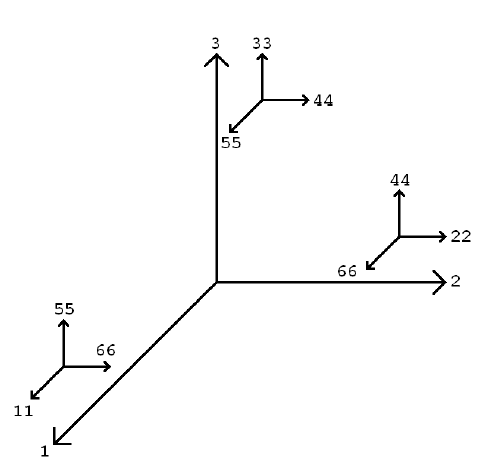
\includegraphics[width=0.5\textwidth]{png/speeds.png}}
\caption{Скорости распространения продольной и двух поперечных волн для каждой квазиодномерной волны.}
\label{pic:speeds-waves}
\end{figure}

\subsubsection{Трансверсальньно изотропное тело}
	
	Следующий тип анизотропии предполагает наличие во всех точках параллельных плоскостей упругой симметрии\cite{lehnitsky}.
	Иначе говоря, в каждой точке есть плоскость все направления в которой эквивалентны, а также есть выделенное направление, нормальное к плоскости.
	
	Примем за выделенное направление множество векторов коллинеарных оси $Z$, тогда плоскости изотропии будут параллельны плоскости $XY$.
	Матрица упругих постоянных имеет в этом случае всего пять независимых компонент:
\begin{align}
\label{vert_trans_tensor}
\left( \begin{array}{cccccccccccc}
c_{11} & c_{12} & c_{13} & 0 & 0 & 0 \\ 
c_{12} & c_{11} & c_{13} & 0 & 0 & 0 \\ 
c_{13} & c_{13} & c_{33} & 0 & 0 & 0 \\ 
0 & 0 & 0 & c_{44} & 0 & 0 \\ 
0 & 0 & 0 & 0 & c_{44} & 0 \\ 
0 & 0 & 0 & 0 & 0 & c_{66}
\end{array} \right){}
\end{align}
	где компоненты $c_{11}$, $c_{12}$, $c_{66}$ связаны соотношением:
\begin{equation}
	c_{66} = \frac{c_{11} - c_{12}}{2}.
\end{equation}

	Тензор упругих постоянных в этом случае похож на его аналог для орторомбической анизотропии, но тут он имеет меньшее количество независимых компонент.
	Это значит, что матрицы $\mathbf{A}_x$, $\mathbf{A}_y$, $\mathbf{A}_z$, а значит и собственные значения и собственные строки, имеют вид \eqref{orthorombic_mat1}-\eqref{orthorombic_mat3} с той лишь разницей, что некоторые компоненты зависимы и выражаются через другие.
	
	Данный вид анизотропии типичен для гексагональных решёток, а также для матрицы, аримированной однонаправленными волокнами -- основы ПКМ.
	
\subsection{Преобразование тензора упругих постоянных при повороте базиса}
	
	Многослойные ПКМ состоят из одинаковых слоёв, по-разному ориентированных вокруг оси укладки композита.
	Для расчёта конструкций необходимо найти вид тензора упругих постоянных в произвольно ориентированном базисе \cite{favorskaya}.
	
	Пусть $\theta_{x}$, $\theta_{y}$, $\theta_{z}$ -- углы поворота вокруг осей $x$, $y$, $z$ соответственно. 
	Чтобы перейти от старого базиса к новому нужно произвести последовательно эти повороты.
	Матрицы поворота будут иметь вид:
\begin{align}
\label{rotation_mat1}
\mathbf{G}_x =
\left( \begin{array}{cccccccccccc}
1 & 0 & 0 \\ 
0 & \cos \theta_{x} & -\sin \theta_{x} \\ 
0 & \sin \theta_{x} & \cos \theta_{x}
\end{array} \right),
\end{align} 
\begin{align}
\label{rotation_mat2}
\mathbf{G}_y =
\left( \begin{array}{cccccccccccc}
\cos \theta_{y} & 0 & \sin \theta_{y} \\
0 & 1 & 0 \\ 
-\sin \theta_{y} & 0 & \cos \theta_{y} 
\end{array} \right),
\end{align}
\begin{align}
\label{rotation_mat3}
\mathbf{G}_z =
\left( \begin{array}{cccccccccccc}
\cos \theta_{z} & -\sin \theta_{z} & 0 \\ 
\sin \theta_{z} & \cos \theta_{z} & 0 \\  
0 & 0 & 1  
\end{array} \right).
\end{align}
	
	Итоговая матрица преобразования базиса $\mathbf{G} = \mathbf{G}_{x}\mathbf{G}_{y}\mathbf{G}_{z}$ имеет вид:
\begin{align}
\label{rotation_mat}
\left( \begin{array}{cccccccccccc}
\cos \theta_{y} \cos \theta_{z} & \cos \theta_{z} \sin \theta_{x} \sin \theta_{y} - \sin \theta_{z} \cos \theta_{x} & \cos \theta_{x} \sin \theta_{y} \cos \theta_{z} + \sin \theta_{x} \sin \theta_{z} \\ 
\cos \theta_{y} \sin \theta_{z} & \sin \theta_{z} \sin \theta_{x} \sin \theta_{y} + \cos \theta_{z} \cos \theta_{x} & \cos \theta_{x} \sin \theta_{y} \sin \theta_{z} - \sin \theta_{x} \cos \theta_{z} \\ 
- \sin \theta_{y} & \sin \theta_{x} \cos \theta_{y} & \cos \theta_{x} \cos \theta_{y}
\end{array} \right)
\end{align}


	В итоге, тензор упругих постоянных $C_{ijkl}$, обсуждаемый в пункте 2.1, при поворотах системы координат будет преобразовываться по закону:
\begin{align}
	C_{mnpq} = \sum_{i,\;j,\;k,\;l = 1}^{3} g_{mi}\;g_{nj}\;g_{pk}\;g_{ql}\;C_{ijkl},
\end{align}
	где $g_{ij}$ -- тензор поворота, соответствующий матрице $\mathbf{G}$.

\clearpage
\newpage
\section*{Глава 3\\Численный метод}
\addcontentsline{toc}{section}{Глава 3. Численный метод}
\setcounter{section}{3}
\setcounter{subsection}{0}
\setcounter{equation}{0}

\subsection{Расщепление по направлениям}

	Чтобы решить систему уравнений:
\begin{equation}
	\label{matrix_anisotropy_equation1}
	\frac{\partial\vec{u}}{\partial{t}}+\mathbf{A}_x\frac{\partial\vec{u}}{\partial{x}}+
	\mathbf{A}_y\frac{\partial\vec{u}}{\partial{y}}+
	\mathbf{A}_z\frac{\partial\vec{u}}{\partial{z}}=0
\end{equation}
	методом конечных разностей потребывалось записать бы это уравнение на некотором сеточном шаблоне в каждом узле сетки, а затем решать полученную линейную систему.
	Решение этой системы, состоящей из огромного количества переменных представляется очень сложной задачей.
	С другой стороны вид системы \eqref{matrix_anisotropy_equation1} позволяет нам применить метод дробных шагов для её решения, сводя её, таким образом, к одномерной постановке:
\begin{equation}
	\label{norm_form}
	\frac{\partial\vec{u}}{\partial{t}}+\mathbf{A}_x\frac{\partial\vec{u}}{\partial{x}} = 0
\end{equation}

	Запишем для уравнения \eqref{norm_form} соотношение между искомым вектором на следующем временном слое $\vec{u}^{n+1}$ и на текущем $\vec{u}^{n}$ через оператор перехода между слоями $f$ в виде:
\begin{equation}
	\label{simple_splitting}
	\vec{u}^{n+1} = f_x(\mathbf{A}_x)\vec{u}^{n}.
\end{equation}	
	
	Тогда, в простейшем случае, окончательные выражение для $\vec{u}^{n+1}$ будет:
\begin{equation}
	\label{simple_3D_splitting}
	\vec{u}^{n+1} = F(\mathbf{A}_x, \mathbf{A}_y, \mathbf{A}_z)\vec{u}^{n},
\end{equation}
\begin{equation}
	\label{simple_3D_split_operator}
	F(\mathbf{A}_x, \mathbf{A}_y, \mathbf{A}_z) = \alpha_x f_x(\frac{\mathbf{A}_x}{\alpha_x}) + \alpha_y f_y(\frac{\mathbf{A}_y}{\alpha_y}) + \alpha_z f_z(\frac{\mathbf{A}_z}{\alpha_z}).
\end{equation}
	
	При условии, что за $f_x$, $f_y$, $f_z$ взяты разностные схемы, аппроксимирующие соответствующие уравнения вида \eqref{norm_form}, как минимум первого порядка точности по пространству, а также при выполнении условия:
\begin{equation}
	\label{simple_3D_split_cond}
	\alpha_x + \alpha_y + \alpha_z = 1, \quad \alpha_x, \alpha_y, \alpha_z > 0,
\end{equation}
	схема \eqref{simple_3D_splitting} с оператором \eqref{simple_3D_split_operator} обеспечивает первый порядок точности.
	Такой подход, комбинирующий сочетания решений одномерных систем, носит название \textit{расщепление по направлениям} \cite{chelnokov}.
	
	Ограничение на шаг по времени $\tau$, обеспечивающее устойчивость дальнейшего численного решения, будет иметь вид:
\begin{equation}
\tau \le \max{\tau_j} = \frac{\min(h)}{\max(|\lambda_j^*|)} = \frac{\min(h)\alpha_j}{\max(|\lambda_j|)},
\end{equation}
	где $\lambda_j$ -- собственные значения матриц $\mathbf{A}_x$, $\mathbf{A}_y$, $\mathbf{A}_z$.
	
	Если за одномерные операторы перехода $f$ взять схемы второго порядка и скомбинировать их в полный оператор:
\begin{equation}
	\label{3D_split_operator}
	F(\mathbf{A}_x, \mathbf{A}_y, \mathbf{A}_z) = \frac{1}{6}\sum_{i \neq j \neq k \neq i} f_i(\mathbf{A}_i)f_j(\mathbf{A}_j)f_k(\mathbf{A}_k),
\end{equation}
	то мы получим схему второго порядка. 
	
	Допустимый шаг по времени определяется минимальным допустимым шагом по времени для схем $f_j$:
\begin{align}
\tau = \min\limits_{j}(\tau_j) = \min\limits_{j}(\frac{\min(h)}{\max(|\lambda_j|)}) = \frac{\min(h)}{\max\limits_{j}\max(|\lambda_j|)}.
\end{align}
	
	Однако вычисления по схеме \eqref{3D_split_operator} требуют больших затрат компьютерного времени и памяти.
	Как оказалось, вычисление любого одного слагаемого из \eqref{3D_split_operator} даёт хорошее приближение к схеме второго порядка, например:	
\begin{equation}
	\label{short_3D_split_operator}
	F(\mathbf{A}_x, \mathbf{A}_y, \mathbf{A}_z) = f_x(\mathbf{A}_x)f_y(\mathbf{A}_y)f_z(\mathbf{A}_z).
\end{equation}
	
\subsection{Гиперболическая система уравнений. Инварианты Римана}
	
	Систему квазилинейных уравнений в частных производных, записанную в \textit{нормальной форме} \eqref{norm_form} будем считать \textit{гиперболической}.
	Это значит, что матрица $\mathbf{A}$ подчиняется условиям\cite{rozhdestvenskiy}:
\begin{itemize}
	\item все собственные значения матрицы $\lambda_{i} = \lambda_{i}(t, x, \vec{u})$, $i = \overline{1, 9}$ вещественны;
	\item система собственных векторов матрицы $\{l_{i}(t, x, \vec{u})\}$, $i = \overline{1, 9}$ образует базис в пространстве $E_{n}$.
\end{itemize}

	В таком случае матрица $\mathbf{A}$ \textit{диагонализуема}, т.е. существует базис -- басиз собственных векторов -- в котором она имеет диагональный вид.
	Тут мы будем говорить о собственных строках $\vec{l}^{T}$, таких, что:
\begin{equation}
	\label{eigenstr_equation}
	\vec{l}^{T}\mathbf{A} = \lambda\vec{l}^{T}.
\end{equation}
	
	Итак, матрица $\mathbf{A}$ представима в виде:
\begin{equation}
	\label{diagonal_view}
	\mathbf{A} = \mathbf{\Omega}^{-1}\mathbf{\Lambda}\mathbf{\Omega},
\end{equation}	
	где $\mathbf{\Omega}$ -- матрица собственных строк, $\mathbf{\Lambda}$ -- диагональная матрица собственных значений.
	Тогда умножая справа \eqref{norm_form} на $\mathbf{\Omega}$ получим:
\begin{equation}
	\label{norm_form1}
	\mathbf{\Omega}\frac{\partial\vec{u}}{\partial{t}}+\mathbf{\Lambda}\mathbf{\Omega}\frac{\partial\vec{u}}{\partial{x}} = 0.
\end{equation}
	Далее, если компоненты матрицы $\mathbf{\Omega}$ не зависят от переменных $(x, t)$, то её можно внести под знак дифференцила:
\begin{equation}
	\label{norm_form2}
	\frac{\partial(\mathbf{\Omega}\vec{u})}{\partial{t}}+\mathbf{\Lambda}\frac{\partial(\mathbf{\Omega}\vec{u})}{\partial{x}} = 0.
\end{equation}
	В общем случае, когда $\mathbf{\Omega} = \mathbf{\Omega}(x, t, \vec{u})$, $\mathbf{\Lambda} = \mathbf{\Lambda}(x, t, \vec{u})$ можно попробывать поискать интегрирующий множитель, однако для системы девяти уравнений это проблематично.
	
	Обозначая, $\vec{r} = \mathbf{\Omega}\vec{u}$ получим уравнение:
\begin{equation}
	\label{Riman_invariantes}
	\frac{\partial\vec{r}}{\partial{t}}+\mathbf{\Lambda}\frac{\partial\vec{r}}{\partial{x}} = 0.
\end{equation}
	Или же в такой форме \cite{kukudzhanov_main}:
\begin{equation}
	\label{Riman_invariantes1}
	\left(\frac{dr_k}{dt}\right)_k = 0, \quad k = \overline{1, 9},
\end{equation}
	где $r_k$, компоненты вектора $\vec{r}$ называются \textit{инвариантами Римана}, а система \eqref{Riman_invariantes} \textit{системой в инвариантах}.
	В записи \eqref{Riman_invariantes} введено обозначение:
\begin{equation}
	\label{notation}
	\left(\frac{d}{dt}\right)_k = \frac{\partial}{\partial{t}} + \lambda_k \frac{\partial}{\partial{x}}
\end{equation}
	Это оператор дифференцирования вдоль направления, заданного уравнением:
\begin{equation}
	\label{characteristic_direction}
	\frac{dx}{dt} = \lambda_k, \quad k = \overline{1, 9}.
\end{equation}
	Уравнения \eqref{characteristic_direction} -- уравнения на \textit{характеристики} системы \eqref{norm_form} -- интегральные кривые вдоль которых инварианты $r_k$ постоянны. 
	
	Эти рассуждения лежат в основе \textit{метода характеристик} -- метода решения систем гиперболических уравнений, в котором решение уравнений в частных производных сводится к решению обыкновенных дифференциальных уравнений (ОДУ).
	В свою очередь, для численного решения ОДУ могут быть применены стандартные конечно-разностные схемы. Такой подход составляет суть \textit{сеточно-характеристического метода}. 
	
\subsection{Cеточно-характериситческий метод}

	Гиперболические уравнения описывают распространение различного типа волн в средах.
	Простейшим решением одномерного волнового уравнения являются две волны: $f(x \pm vt)$, распространяющиеся в противоположных направлениях.
	Функция $f$ -- вид начального возмущения, как можно видеть, параметризованная указаным образом, она даёт решение уравнения.
	Важным здесь является то, что некоторые линейные комбинации искомых величин сохраняются на определённых пространственно-временных кривых (характеристиках).

\begin{figure}[H]
	\center{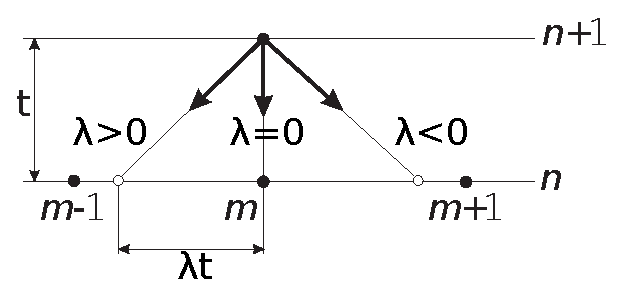
\includegraphics[width=0.5\textwidth]{png/gcm-idea.eps}}
	\caption{Принципиальная схема сеточно-характеристического метода.}
\end{figure}

	После расщепления наша система предстаёт в виде трёх гиперболических систем, описывающих распространение продольной и двух поперечных волн вдоль каждой оси (всего вдоль каждой оси распространяется шесть волн -- с положительными и отрицательными скоростями).
	Затем, переходя к инвариантам, мы получаем девять уравнений переноса вдоль каждой оси.
	Решение этих уравнений сеточно-характеристическим методом осуществляемся следующим образом:
\begin{enumerate}
	\item Из узлов сетки на очередном временном слое проводятся характеристики на предыдущий временной слой (см. Рис. 2). Для линейной системы уравнений характеристиками будут семейства параллельных прямых.
	\item Находятся точки пересечения характеристик с предыдущим временным слоем.
	\item В этих точках, применяя различные схемы, производится интерполяция искомых функций (на Рис. 2 изображён трёхточечный шаблон).
	\item По найденным значениям производится пересчёт инвариантов, которые переносятся по характеристикам в исходный узел.
\end{enumerate}
	
	Как уже сказано характеристики -- прямые линиии постоянного наклона. Это значит можно точно решить уравнение на характеристики \eqref{characteristic_direction}, поэтому определяющим фактором здесь является интреполяция инвариантов.
	Схема интерполяции второго порядка с разностями против потока (upwind scheme) является здесь предпочтительной.
	При числе Куранта в близкой окрестности единицы эта схема может оказаться особенной точной.
	
	В итоге инварианты на $(n+1)$-ом временном слое можно записать в виде:
\begin{equation}
	r_{i}^{n+1} = r_{i}^{n}(- \lambda_{i}\tau),
\end{equation}
	где $r_{i}$ -- $i$-ый инвариант Римана, $\lambda_{i}$ -- соответствующее ему собственное значение.
	Такая запись означает, что значение инварианта $r_{i}$ берётся на $n$-ом слое в точке смёщённой на $-\lambda_{i}\tau$ от координаты искомой.
	
	Затем искомый $\vec{u}$ вектор находится по формуле:
\begin{equation}
	\vec{u} = \mathbf{\Omega^{-1}}\vec{r}.
\end{equation}	

\subsection{Разностные схемы для структурированных сеток}
	
	Существует множество готовых расностных схем для решения уравнения \eqref{norm_form}.
	По сути эти схемы аналогичны сеточно-характерестическому методу, использующему различные схемы интерполяции инвариантов на предыдущем слое.
	
\paragraph{Схема Куранта-Изаксона-Рис.} Данная схема строится на трёхточечном сеточном шаблоне $(m-1, m, m+1)$ и позволяет явно выразить значение $\vec{u}_m^{n+1}$ на новом временном слое:
\begin{equation}
	\label{CIR scheme}
	\vec{u}^{n+1}_m = \vec{u}^n_m - \frac{\tau}{h} \mathbf{\Omega}^{-1} \mathbf{\Lambda}^+ \mathbf{\Omega} (\vec{u}^n_{m+1} - \vec{u}^n_m) 
	- \frac{\tau}{h} \mathbf{\Omega}^{-1} \mathbf{\Lambda}^- \mathbf{\Omega} (\vec{u}^n_m - \vec{u}^n_{m-1}) .
\end{equation}
	Здесь диагональные матрицы $\mathbf{\Lambda}^+$, $\mathbf{\Lambda}^-$ содержат соответственно положительные и отрицательные собственные значения (скорости распространения волн).
	
	Эта схема является схемой первого порядка точности по времени и пространству -- $O(h, \tau)$.
	
\paragraph{Схема Лакса-Вендрофа.} Стандартная схема Лакса-Вендрофа обладает вторым порядком точности и по времени и по пространству -- $O(h^2 + \tau^2)$.
\begin{equation}
	\label{LW scheme}
	\vec{u}^{n+1}_m = \vec{u}^n_m - \frac{\tau}{2h} \mathbf{A} (\vec{u}^n_{m+1} - \vec{u}^n_{m-1})
	 + \frac{\tau^2}{2h^2} \mathbf{A}^2 (\vec{u}^n_{m+1} - 2\vec{u}^n_m + \vec{u}^n_{m-1}) .
\end{equation}
	Эта схема в отличие от предыдущей не является монотонной. 
	Схемы, у которых отсутствует свойство монотонности плохо аппроксимируют решения с большими градиентами -- они выдают осцилляции разностного происхождения вблизи области с больши градиентом.
	
\paragraph{Гибридная схема.} Именно для сочетания точности схем второго порядка и устранения осцилляций для решений с большими градиентами Р.П. Федоренко впервые предложил \textit{гибридные схемы} \cite{fedorenko}.
	В нашем случае, комбинируя схему \eqref{CIR scheme} со схемой \eqref{LW scheme}, итоговое решение будет иметь вид линейной комбинации решений двух схем:
\begin{align}
	\label{hybrid scheme}
	\vec{u}^{n+1}_m &= \vec{u}^n_m - \frac{\tau}{2h} \mathbf{A} (\vec{u}^n_{m+1} - \vec{u}^n_{m-1}) + \nonumber\\
		&+ \frac{1}{2} ((1-a) \frac{\tau}{h} \mathbf{\Omega}^{-1} |\mathbf{\Lambda}| \mathbf{\Omega} + a \frac{\tau^2}{h^2} \mathbf{A}^2 ) (\vec{u}^n_{m+1} - 2\vec{u}^n_m + \vec{u}^n_{m-1}).
\end{align}
	Параметр $a$ может принимать значения: $0 \leq a \leq 1$, и подбирается на каждом шагу в зависимости от степени гладкости решения. 
	В случае $a = 0$ схема \eqref{hybrid scheme} переходит в схему Куранта-Изаксона-Рис \eqref{CIR scheme}.
	В случае $a = 1$ схема \eqref{hybrid scheme} переходит в схему Лакса-Вендрофа \eqref{LW scheme}.
	
	Решение уравнения \eqref{norm_form} по схеме \eqref{hybrid scheme} заключается в переключении между схемами \eqref{CIR scheme} и \eqref{LW scheme} в зависимости от гладкости $n$-ого временного слоя.
	Критерий переключения имеет вид:
\begin{equation}
	\label{Fedorenko criterium}
	\left|\frac{\vec{u}^n_{m+1} - 2\vec{u}^n_m + \vec{u}^n_{m-1}}{\vec{u}^n_{m+1} - \vec{u}^n_{m-1}}\right| \le K,
\end{equation}
	где параметр переключения -- $K$ подбирается, опять же, в зависимости от гладкости решения и в данной работе: $K = 0.5$.
	В случае выполнения условия \eqref{Fedorenko criterium} решение считается достаточно гладким, параметр принимает значение: $a = 1$ и расчёт ведётся по схеме Лакса-Вендрофа.
	Если же критерий не выполняется, то $a = 0$ и расчёт производится по схеме Куранта-Изаксона-Рис.
	
	На Рис. 3 изображены несколько численных решений распространения прямоугольного импульса. Как можно отметить гибридная схема лучше остальных приближает точное решение.
\begin{figure}[H]
\centerline{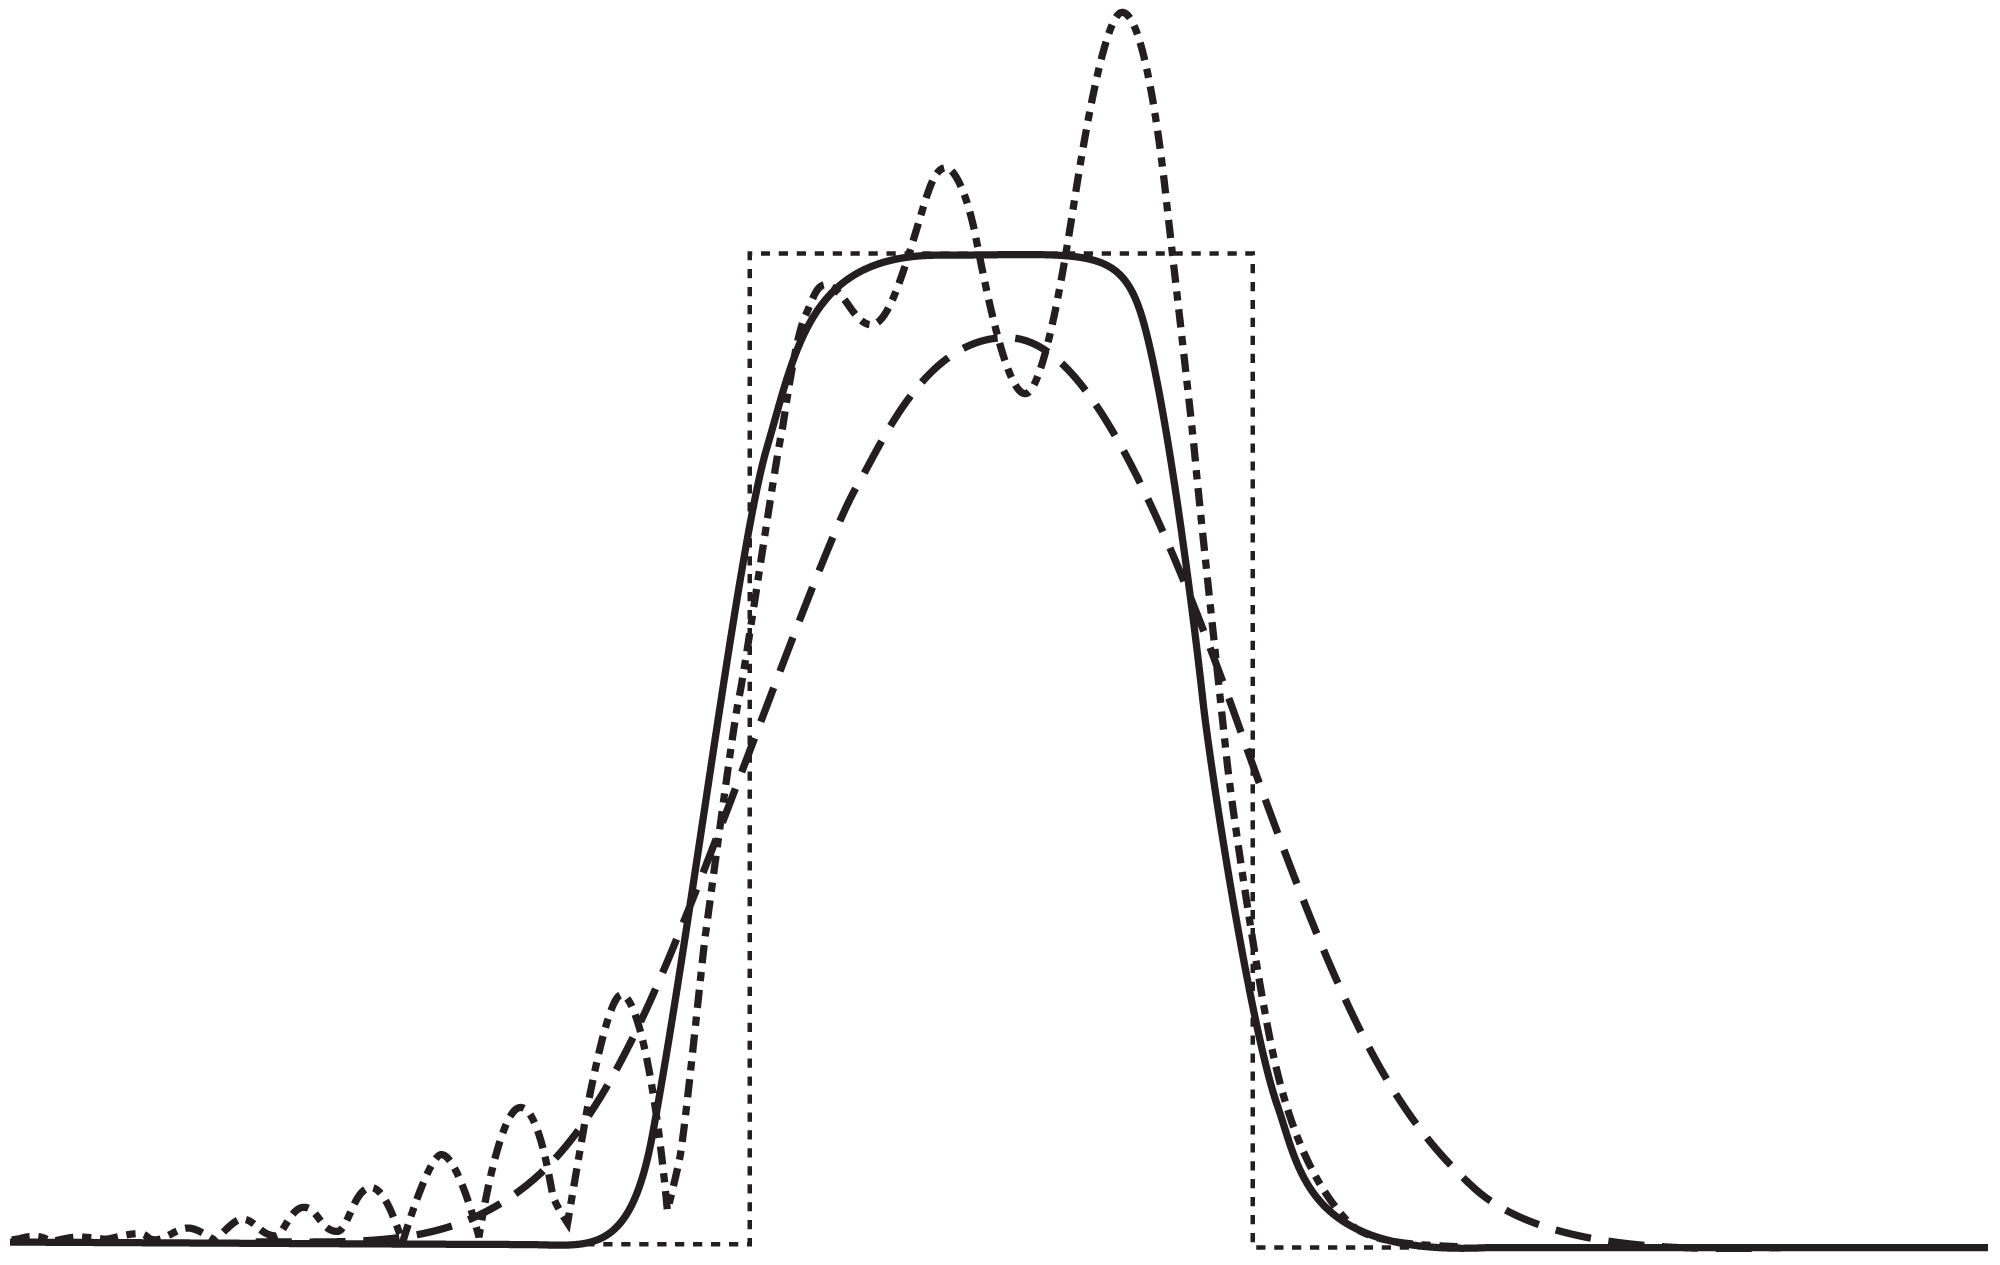
\includegraphics[width=0.75\textwidth]{png/hybrid-scheme-testing.png}}
\caption{Распространение прямоугольного импульса. Штриховая линия -- решение по схеме Куранта-Изаксона-Рис. Штрих-пунктирная -- решение по схеме Лакса-Вендрофа. Сплошная линия -- решение с использованием гибридной схемы. Точками показано точное решение.}
\label{pic:hybrid-scheme-testing}
\end{figure}

\clearpage
\newpage
\section*{Глава 4\\Результаты расчётов}
\addcontentsline{toc}{section}{Глава 4. Результаты расчётов}
\setcounter{section}{4}
\setcounter{subsection}{0}
\setcounter{equation}{0}

\subsection{Верификация}

	В общем виде система линеных гиперболических уравнений \eqref{matrix_anisotropy_equation1} не решена и не доказана теорема существования её решения.
	Более того пока ещё не построено решение одномерной системы \eqref{norm_form}, получающейся после расщепления, для произвольного вида границы.
	Тем не менее после перехода к инвариантам система распадается на девять уравнений переноса, для которых известно аналитическое решение.
	Воспользуемся этим решением для проверки численного метода в простейшем случае \textbf{P} и \textbf{S} волн.

\subsubsection{P, S - волны}

	\textit{P-волной} называется продольная упругая волна, т.е. волна у которой вектор распространения параллелен вектору поляризации.
	\textit{S-волна} -- поперечная упругая волна. Для нёё вектор распространения перпендикулярен вектору поляризации.
	
	Рассмотрим, как задать P и S волны для уравнения:
\begin{equation}
	\label{norm_form_results}
	\frac{\partial\vec{u}}{\partial{t}}+\mathbf{A}_z\frac{\partial\vec{u}}{\partial{z}}=0.
\end{equation}
	
	Пусть материал будет \textit{ортотропным}, тогда матрица упругих постоянных будет выглядеть следующим образом:
\begin{align}
\label{orthorombic_tensor}
\left( \begin{array}{cccccccccccc}
c_{11} & c_{12} & c_{13} & 0 & 0 & 0 \\ 
c_{12} & c_{22} & c_{23} & 0 & 0 & 0 \\ 
c_{13} & c_{23} & c_{33} & 0 & 0 & 0 \\ 
0 & 0 & 0 & c_{44} & 0 & 0 \\ 
0 & 0 & 0 & 0 & c_{55} & 0 \\ 
0 & 0 & 0 & 0 & 0 & c_{66}
\end{array} \right){}
\end{align}	
	Собственные значения для матрицы $\mathbf{A}_z$ в таком случае имеют вид:	
\begin{align}
	\left\{0,\;0,\;0,\;\sqrt{\frac{c_{33}}{\rho}},\;\sqrt{\frac{c_{44}}{\rho}},\;\sqrt{\frac{c_{55}}{\rho}},\;-\sqrt{\frac{c_{33}}{\rho}},\;-\sqrt{\frac{c_{44}}{\rho}},\;-\sqrt{\frac{c_{55}}{\rho}}\right\}.
\end{align}
	Инварианты Римана для уравнения \eqref{norm_form_results} можно записать $\vec{r} = \mathbf{\Omega}_z\vec{u}$ или покомпонентно:
\begin{align}
\label{Z_invariants}
\vec{r} =
\left( \begin{array}{cccccccccccc}
0 & 0 & 0 & 1 & 0 & 0 & 0 & 0 & -\frac{c_{13}}{c_{33}} \\ 
0 & 0 & 0 & 0 & 1 & 0 & 0 & 0 & 0 \\ 
0 & 0 & 0 & 0 & 0 & 0 & 1 & 0 & -\frac{c_{23}}{c_{33}} \\ 
0 & 0 & -\sqrt{c_{33}\rho} & 0 & 0 & 0 & 0 & 0 & 1 \\ 
0 & -\sqrt{c_{44}\rho} & 0 & 0 & 0 & 0 & 0 & 1 & 0 \\
-\sqrt{c_{55}\rho} & 0 & 0 & 0 & 0 & 1 & 0 & 0 & 0 \\
0 & 0 & \sqrt{c_{33}\rho} & 0 & 0 & 0 & 0 & 0 & 1 \\ 
0 & \sqrt{c_{44}\rho} & 0 & 0 & 0 & 0 & 0 & 1 & 0 \\
\sqrt{c_{55}\rho} & 0 & 0 & 0 & 0 & 1 & 0 & 0 & 0
\end{array} \right)
\left( \begin{array}{cccccccccccc}
v_x \\
v_y \\
v_z \\
\sigma_{xx} \\
\sigma_{xy} \\
\sigma_{xz} \\
\sigma_{yy} \\
\sigma_{yz} \\
\sigma_{zz}
\end{array} \right).
\end{align}
	
	Для создания P-волны вдоль направления $Z$ следует занулить все инварианты кроме инварианта, соответствующего продольной волне, т.е. кроме строчки в \eqref{Z_invariants}, соответствующей собственному значению $-\sqrt{\frac{c_{33}}{\rho}}$ (знак минус выбран для удобства).
	Потребуем зануления всех инвариантов, кроме седьмой строчки:
\begin{align}	
	\label{p_cond}
	\left\{
		\begin{array}{cccccccccccc}
			c_{33}\sigma_{xx} = c_{13}\sigma_{zz} \\
			\sigma_{xy} = 0 \\
			c_{33}\sigma_{yy} = c_{23}\sigma_{zz} \\
			v_z\sqrt{c_{33}\rho} = \sigma_{zz} \\
			\pm v_y\sqrt{c_{44}\rho} = \sigma_{yz} \\
			\pm v_x\sqrt{c_{55}\rho} = \sigma_{xz}
		\end{array}
	\right.
\end{align}
	Задав начальные значения неизвестных в соответствии с \eqref{p_cond}, получим P-волну в этом направлении.
	
	Аналогично можно выписать соотношения, задающие S-волну для уравнения переноса \eqref{norm_form_results}.
	Скорость распространения поперечной волны вдоль оси $X$ будет $-\sqrt{\frac{c_{55}}{\rho}}$, занулив все инварианты кроме последней строчки в \eqref{Z_invariants}, получим:
\begin{align}	
	\label{s_cond1}
	\left\{
		\begin{array}{cccccccccccc}
			c_{33}\sigma_{xx} = c_{13}\sigma_{zz} \\
			\sigma_{xy} = 0 \\
			c_{33}\sigma_{yy} = c_{23}\sigma_{zz} \\
			\pm v_z\sqrt{c_{33}\rho} = \sigma_{zz} \\
			\pm v_y\sqrt{c_{44}\rho} = \sigma_{yz} \\
			v_x\sqrt{c_{55}\rho} = \sigma_{xz}
		\end{array}
	\right.
\end{align}

	И для поперечной S-волны для \eqref{norm_form_results} вдоль оси $Y$, распространяющейся со скоростью $-\sqrt{\frac{c_{44}}{\rho}}$ имеем:
\begin{align}	
	\label{s_cond2}
	\left\{
		\begin{array}{cccccccccccc}
			c_{33}\sigma_{xx} = c_{13}\sigma_{zz} \\
			\sigma_{xy} = 0 \\
			c_{33}\sigma_{yy} = c_{23}\sigma_{zz} \\
			\pm v_z\sqrt{c_{33}\rho} = \sigma_{zz} \\
			v_y\sqrt{c_{44}\rho} = \sigma_{yz} \\
			\pm v_x\sqrt{c_{55}\rho} = \sigma_{xz}
		\end{array}
	\right.
\end{align}

	Для остальных уравнений вида \eqref{norm_form_results} расщеплённой системы P и S волны задаются по аналогии.
	
\subsubsection{Результаты тестовых расчётов}

	В процессе выполнения работы была произведена модификация пакета программ, предназначенного для численного моделирования динамических процессов распространения механических деформаций в твёрдых телах сеточно-характеристическим методом с явным выделением контакта, для поддержки расчёта анизотропных тел.

	Для проверки созданной модификации были написаны функциональные тесты, сравнивающие численное решение распространения P и S волн в одномерной проекции, а также таски (задания расчётов), создающие эти волны.
	
	За модельный был взят трансверсально-изотропный материал с матрицей упругих постоянных:
\begin{align}
\label{veryfication_mat}
\left( \begin{array}{cccccccccccc}
90000 & 70000 & 17500 & 0 & 0 & 0 \\ 
70000 & 90000 & 17500 & 0 & 0 & 0 \\ 
17500 & 17500 & 22500 & 0 & 0 & 0 \\ 
0 & 0 & 0 & 10000 & 0 & 0 \\ 
0 & 0 & 0 & 0 & 10000 & 0 \\ 
0 & 0 & 0 & 0 & 0 & 10000
\end{array} \right),
\end{align}	
	и условной плотностью равной:
\begin{equation}
	\rho = 1.
\end{equation}
	Все указанные числа обезразмерены.
	Единицу измерения им можно придать задав единицу измерения времени (шаг метода) и единицу измерения длины (размер тела).

	Общий трёхмерный вид всех P и S возмущений представлен на рисунке снизу.
\begin{figure}[H]
\centerline{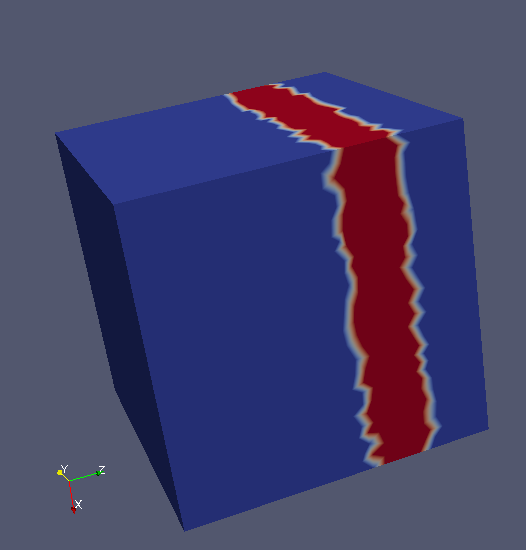
\includegraphics[width=0.4\textwidth]{png/veryfication/p-wave-view.png}}
\caption{Общий трёхмерный вид всех P, S волн. Цветовой гаммой выделена амплитуда скорости.}
\label{pic:p-wave-view}
\end{figure}
	
	Ниже представлены рисунки сравнения численного и аналитического решений для P и S волн уравнения переноса с матрицами $\mathbf{A}_x$, $\mathbf{A}_z$ на различных мелкостях сетки.
	Плоскость $XY$ изотропна, поэтому в ней можно провести проверку в одном направлении.
\begin{figure}[H]
\begin{subfigure}[b]{0.5\textwidth}
\centering
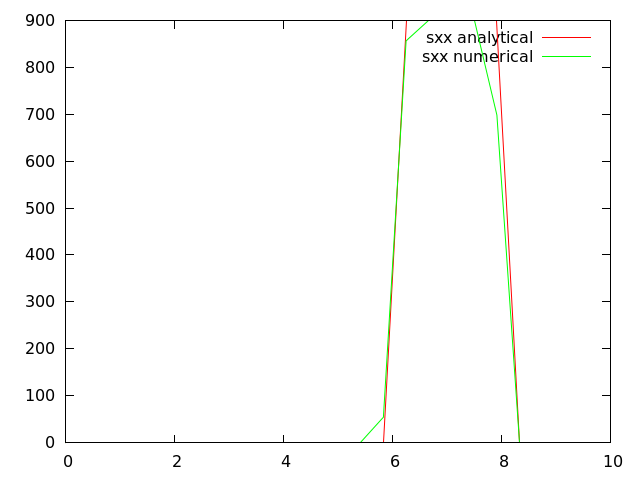
\includegraphics[width=0.75\textwidth]{png/veryfication/0.8/p-wave-along-x0.png}
\caption{Начальное состояние}
\end{subfigure}
\begin{subfigure}[b]{0.5\textwidth}
\centering
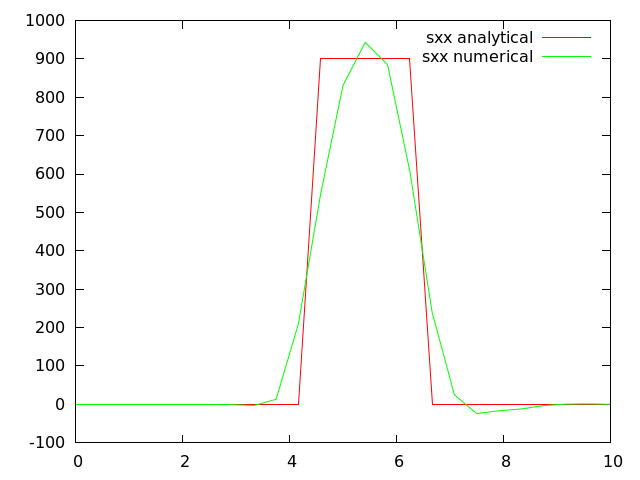
\includegraphics[width=0.75\textwidth]{png/veryfication/0.8/p-wave-along-x5.png}
\caption{5-ый шаг}
\end{subfigure}
\begin{subfigure}[b]{0.5\textwidth}
\centering
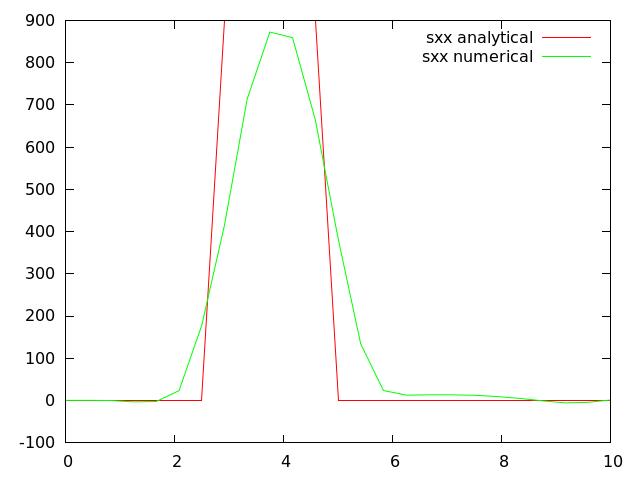
\includegraphics[width=0.75\textwidth]{png/veryfication/0.8/p-wave-along-x10.png}
\caption{10-ый шаг}
\end{subfigure}
\begin{subfigure}[b]{0.5\textwidth}
\centering
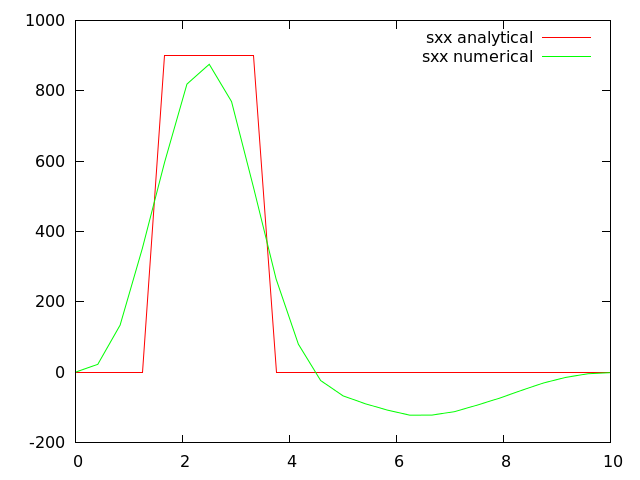
\includegraphics[width=0.75\textwidth]{png/veryfication/0.8/p-wave-along-x15.png}
\caption{15-ый шаг}
\end{subfigure}
\caption{Распространение P-волны вдоль оси $X$. Показана $\sigma_{xx}$ компонента. Размер тетраэдра -- 0.8, шаг по времени -- 0.001025. }
\label{pic:p_wave_along_x8}
\end{figure}

\begin{figure}[H]
\begin{subfigure}[b]{0.5\textwidth}
\centering
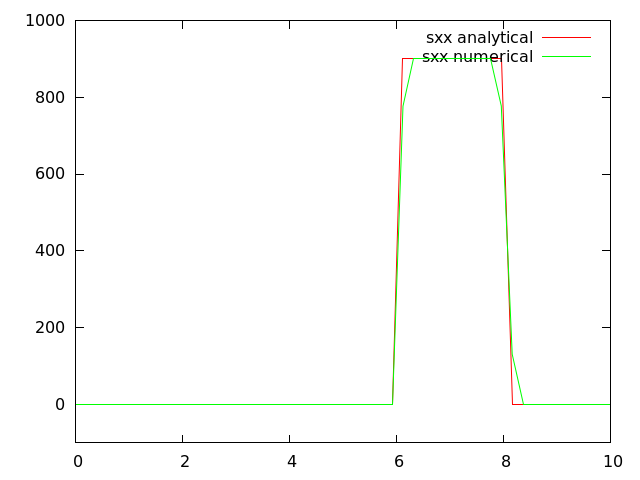
\includegraphics[width=0.75\textwidth]{png/veryfication/0.4/p-wave-along-x0.png}
\caption{Начальное состояние}
\end{subfigure}
\begin{subfigure}[b]{0.5\textwidth}
\centering
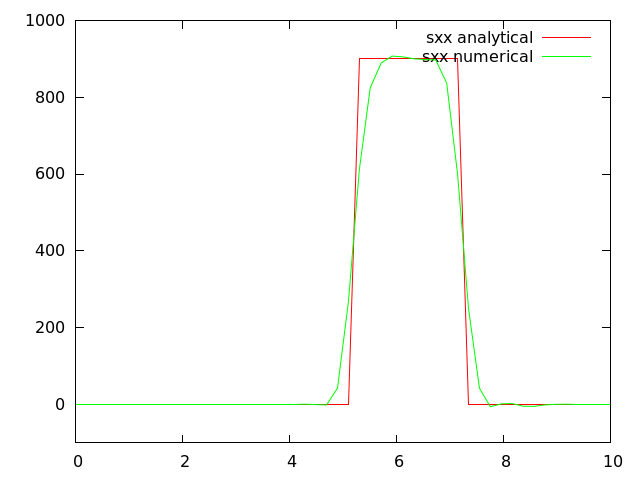
\includegraphics[width=0.75\textwidth]{png/veryfication/0.4/p-wave-along-x5.png}
\caption{5-ый шаг}
\end{subfigure}
\begin{subfigure}[b]{0.5\textwidth}
\centering
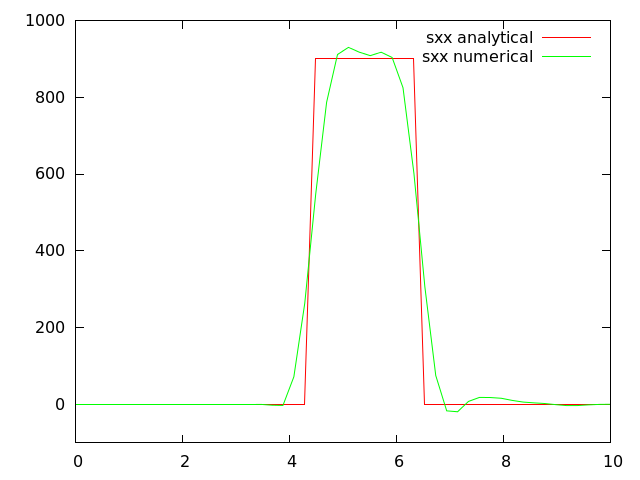
\includegraphics[width=0.75\textwidth]{png/veryfication/0.4/p-wave-along-x10.png}
\caption{10-ый шаг}
\end{subfigure}
\begin{subfigure}[b]{0.5\textwidth}
\centering
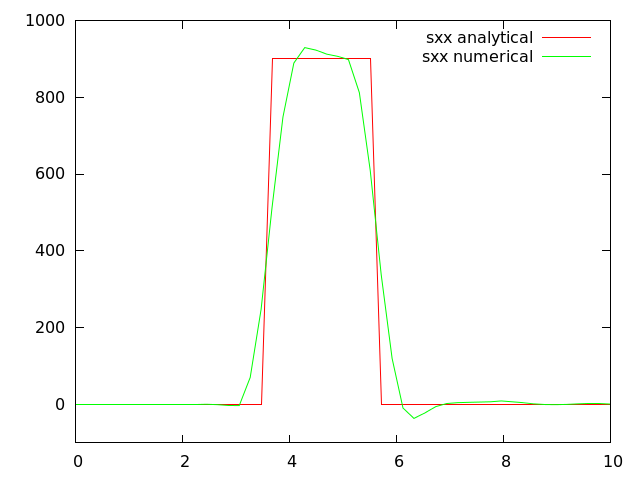
\includegraphics[width=0.75\textwidth]{png/veryfication/0.4/p-wave-along-x15.png}
\caption{15-ый шаг}
\end{subfigure}
\caption{Распространение P-волны вдоль оси $X$. Показана $\sigma_{xx}$ компонента. Размер тетраэдра -- 0.4, шаг по времени -- 0.000533. }
\label{pic:p_wave_along_x4}
\end{figure}

\begin{figure}[H]
\begin{subfigure}[b]{0.5\textwidth}
\centering
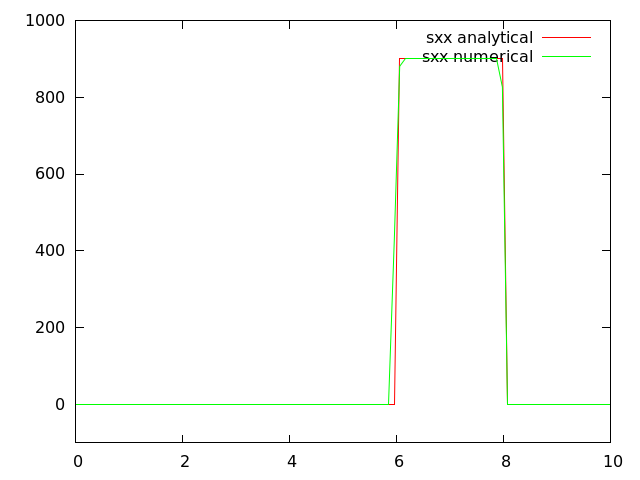
\includegraphics[width=0.75\textwidth]{png/veryfication/0.2/p-wave-along-x0.png}
\caption{Начальное состояние}
\end{subfigure}
\begin{subfigure}[b]{0.5\textwidth}
\centering
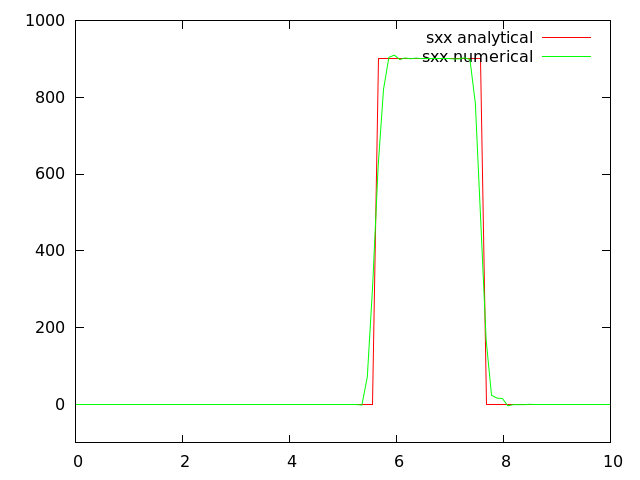
\includegraphics[width=0.75\textwidth]{png/veryfication/0.2/p-wave-along-x5.png}
\caption{5-ый шаг}
\end{subfigure}
\begin{subfigure}[b]{0.5\textwidth}
\centering
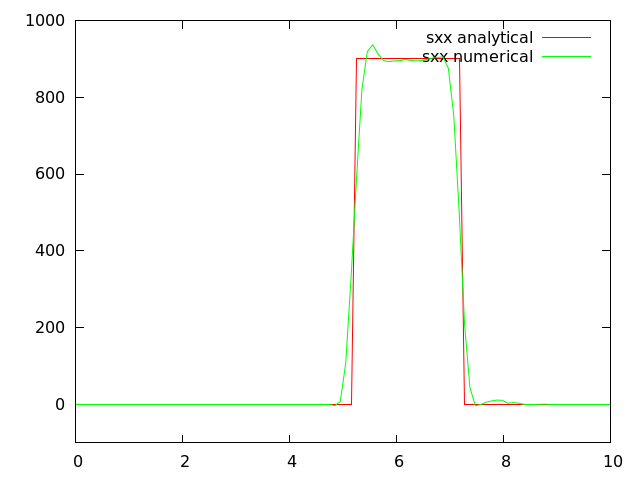
\includegraphics[width=0.75\textwidth]{png/veryfication/0.2/p-wave-along-x10.png}
\caption{10-ый шаг}
\end{subfigure}
\begin{subfigure}[b]{0.5\textwidth}
\centering
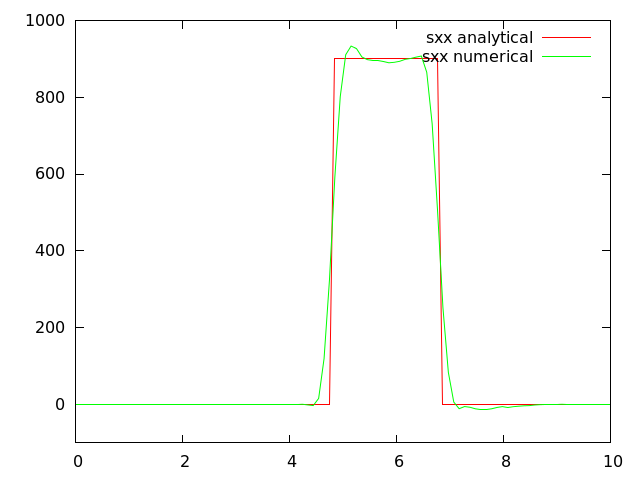
\includegraphics[width=0.75\textwidth]{png/veryfication/0.2/p-wave-along-x15.png}
\caption{15-ый шаг}
\end{subfigure}
\caption{Распространение P-волны вдоль оси $X$. Показана $\sigma_{xx}$ компонента. Размер тетраэдра -- 0.2, шаг по времени -- 0.000269. }
\label{pic:p_wave_along_x2}
\end{figure}

\begin{figure}[H]
\begin{subfigure}[b]{0.5\textwidth}
\centering
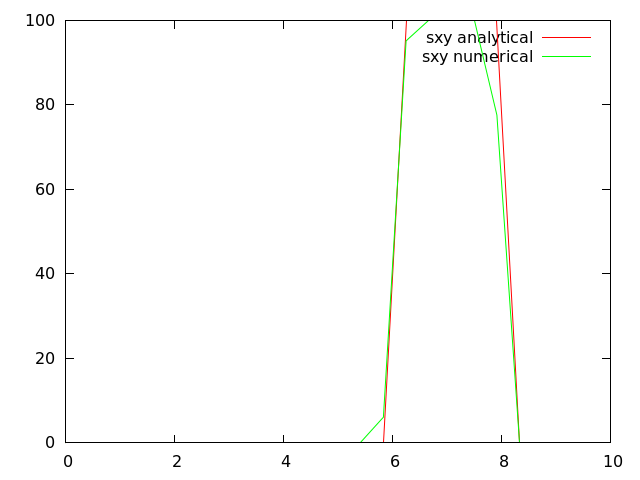
\includegraphics[width=0.75\textwidth]{png/veryfication/0.8/s-wave-along-x0.png}
\caption{Начальное состояние}
\end{subfigure}
\begin{subfigure}[b]{0.5\textwidth}
\centering
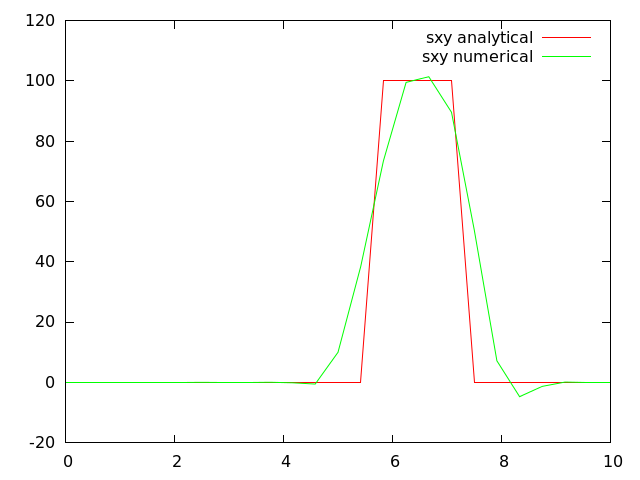
\includegraphics[width=0.75\textwidth]{png/veryfication/0.8/s-wave-along-x5.png}
\caption{5-ый шаг}
\end{subfigure}
\begin{subfigure}[b]{0.5\textwidth}
\centering
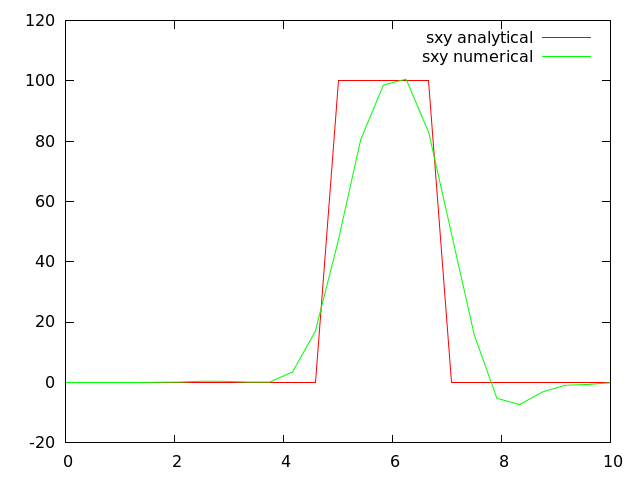
\includegraphics[width=0.75\textwidth]{png/veryfication/0.8/s-wave-along-x10.png}
\caption{10-ый шаг}
\end{subfigure}
\begin{subfigure}[b]{0.5\textwidth}
\centering
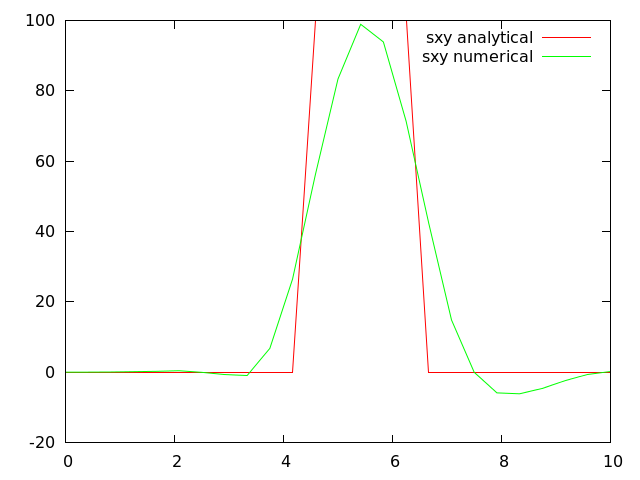
\includegraphics[width=0.75\textwidth]{png/veryfication/0.8/s-wave-along-x15.png}
\caption{15-ый шаг}
\end{subfigure}
\caption{Распространение S-волны вдоль оси $X$. Показана $\sigma_{xy}$ компонента. Размер тетраэдра -- 0.8, шаг по времени -- 0.001025. }
\label{pic:s_wave_along_x8}
\end{figure}

\begin{figure}[H]
\begin{subfigure}[b]{0.5\textwidth}
\centering
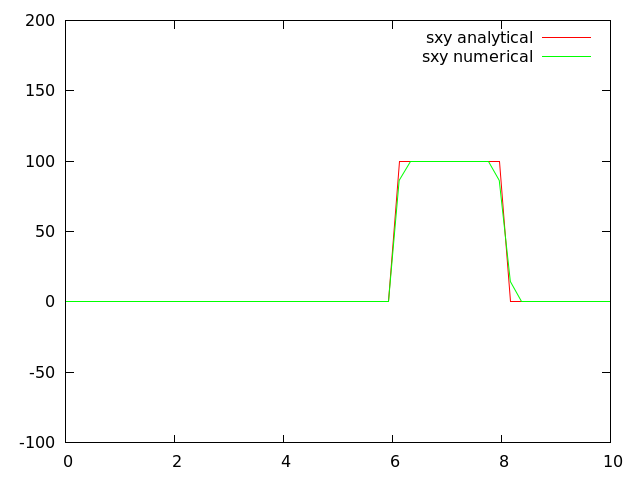
\includegraphics[width=0.75\textwidth]{png/veryfication/0.4/s-wave-along-x0.png}
\caption{Начальное состояние}
\end{subfigure}
\begin{subfigure}[b]{0.5\textwidth}
\centering
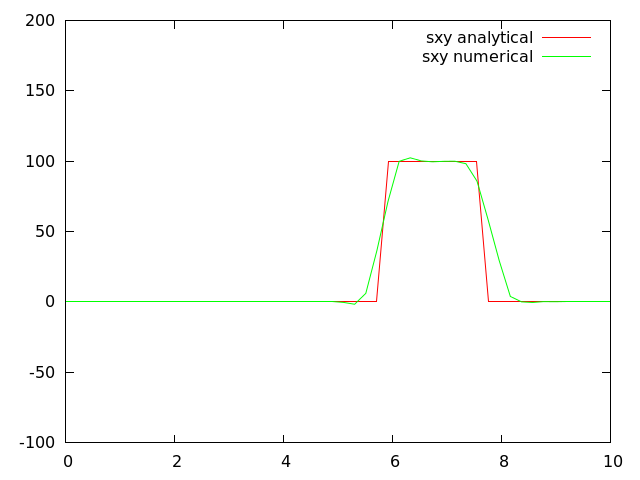
\includegraphics[width=0.75\textwidth]{png/veryfication/0.4/s-wave-along-x5.png}
\caption{5-ый шаг}
\end{subfigure}
\begin{subfigure}[b]{0.5\textwidth}
\centering
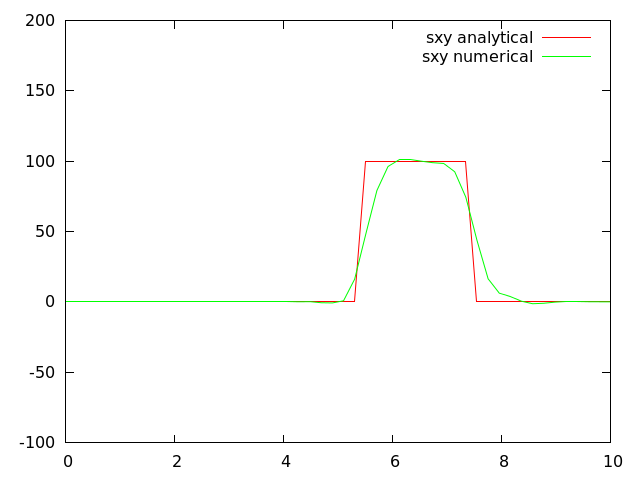
\includegraphics[width=0.75\textwidth]{png/veryfication/0.4/s-wave-along-x10.png}
\caption{10-ый шаг}
\end{subfigure}
\begin{subfigure}[b]{0.5\textwidth}
\centering
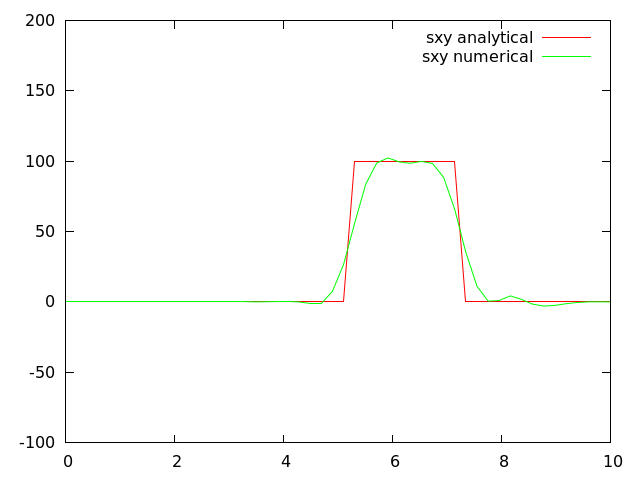
\includegraphics[width=0.75\textwidth]{png/veryfication/0.4/s-wave-along-x15.png}
\caption{15-ый шаг}
\end{subfigure}
\caption{Распространение S-волны вдоль оси $X$. Показана $\sigma_{xy}$ компонента. Размер тетраэдра -- 0.4, шаг по времени -- 0.000533. }
\label{pic:s_wave_along_x4}
\end{figure}

\begin{figure}[H]
\begin{subfigure}[b]{0.5\textwidth}
\centering
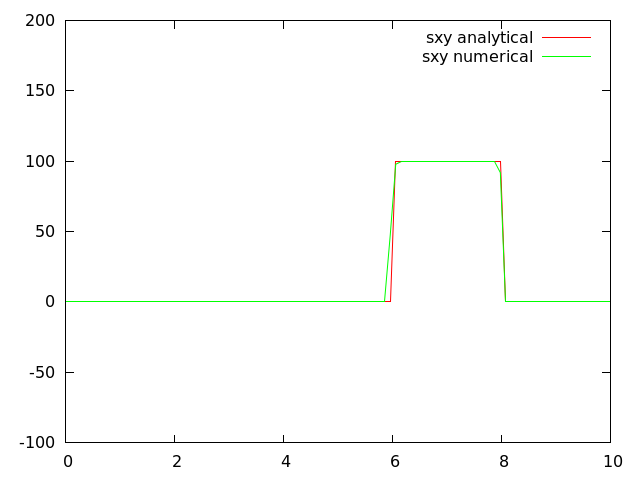
\includegraphics[width=0.75\textwidth]{png/veryfication/0.2/s-wave-along-x0.png}
\caption{Начальное состояние}
\end{subfigure}
\begin{subfigure}[b]{0.5\textwidth}
\centering
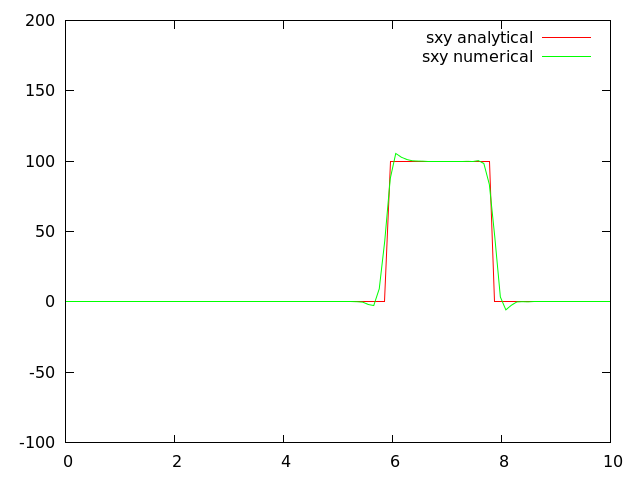
\includegraphics[width=0.75\textwidth]{png/veryfication/0.2/s-wave-along-x5.png}
\caption{5-ый шаг}
\end{subfigure}
\begin{subfigure}[b]{0.5\textwidth}
\centering
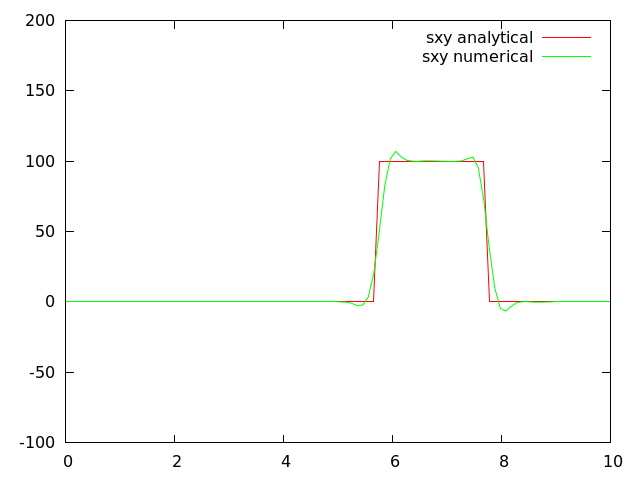
\includegraphics[width=0.75\textwidth]{png/veryfication/0.2/s-wave-along-x10.png}
\caption{10-ый шаг}
\end{subfigure}
\begin{subfigure}[b]{0.5\textwidth}
\centering
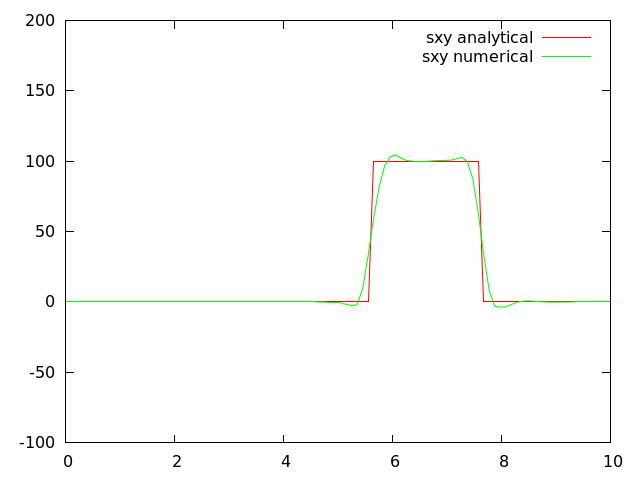
\includegraphics[width=0.75\textwidth]{png/veryfication/0.2/s-wave-along-x15.png}
\caption{15-ый шаг}
\end{subfigure}
\caption{Распространение S-волны вдоль оси $X$. Показана $\sigma_{xy}$ компонента. Размер тетраэдра -- 0.2, шаг по времени -- 0.000269. }
\label{pic:s_wave_along_x2}
\end{figure}

\begin{figure}[H]
\begin{subfigure}[b]{0.5\textwidth}
\centering
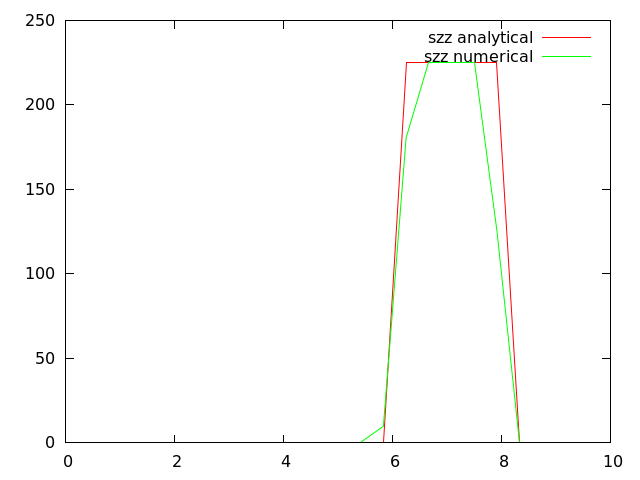
\includegraphics[width=0.75\textwidth]{png/veryfication/0.8/p-wave-along-z0.png}
\caption{Начальное состояние}
\end{subfigure}
\begin{subfigure}[b]{0.5\textwidth}
\centering
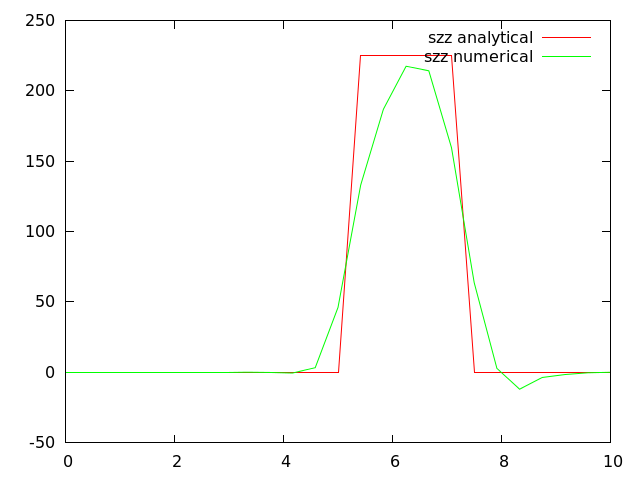
\includegraphics[width=0.75\textwidth]{png/veryfication/0.8/p-wave-along-z5.png}
\caption{5-ый шаг}
\end{subfigure}
\begin{subfigure}[b]{0.5\textwidth}
\centering
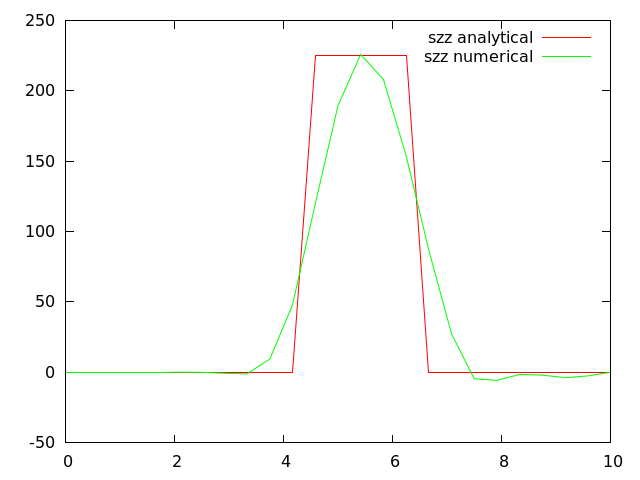
\includegraphics[width=0.75\textwidth]{png/veryfication/0.8/p-wave-along-z10.png}
\caption{10-ый шаг}
\end{subfigure}
\begin{subfigure}[b]{0.5\textwidth}
\centering
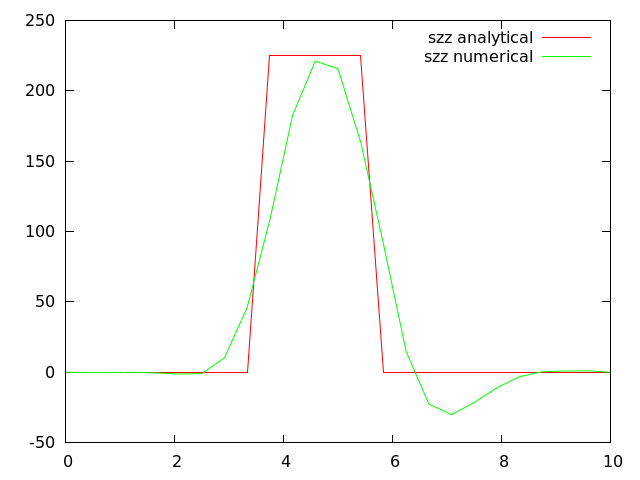
\includegraphics[width=0.75\textwidth]{png/veryfication/0.8/p-wave-along-z15.png}
\caption{15-ый шаг}
\end{subfigure}
\caption{Распространение P-волны вдоль оси $Z$. Показана $\sigma_{zz}$ компонента. Размер тетраэдра -- 0.8, шаг по времени -- 0.001025. }
\label{pic:p_wave_along_z8}
\end{figure}

\begin{figure}[H]
\begin{subfigure}[b]{0.5\textwidth}
\centering
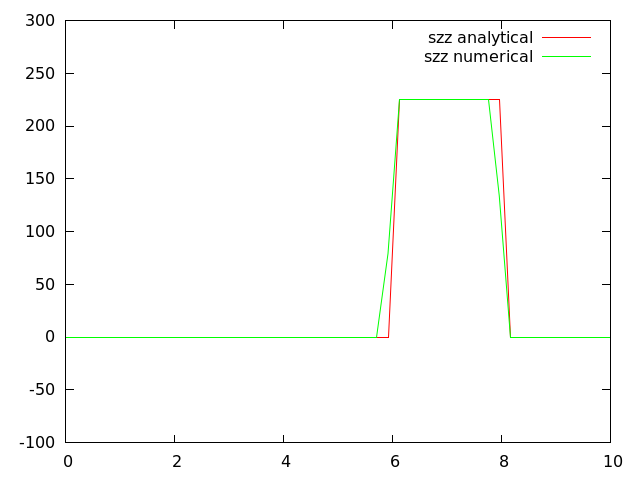
\includegraphics[width=0.75\textwidth]{png/veryfication/0.4/p-wave-along-z0.png}
\caption{Начальное состояние}
\end{subfigure}
\begin{subfigure}[b]{0.5\textwidth}
\centering
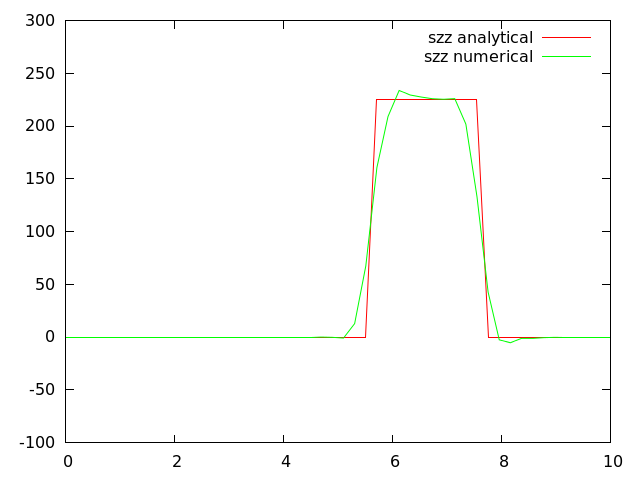
\includegraphics[width=0.75\textwidth]{png/veryfication/0.4/p-wave-along-z5.png}
\caption{5-ый шаг}
\end{subfigure}
\begin{subfigure}[b]{0.5\textwidth}
\centering
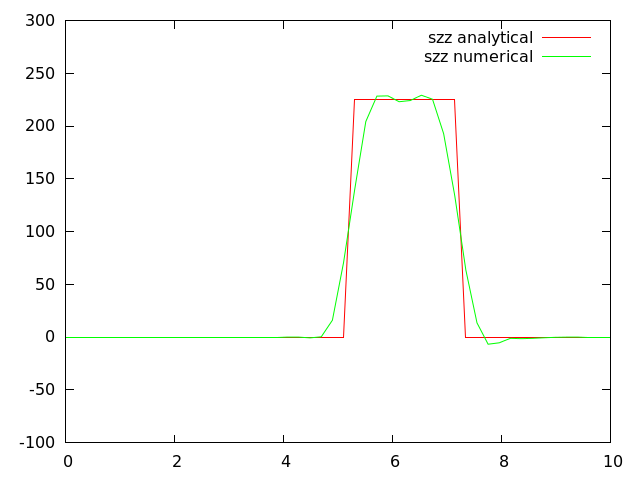
\includegraphics[width=0.75\textwidth]{png/veryfication/0.4/p-wave-along-z10.png}
\caption{10-ый шаг}
\end{subfigure}
\begin{subfigure}[b]{0.5\textwidth}
\centering
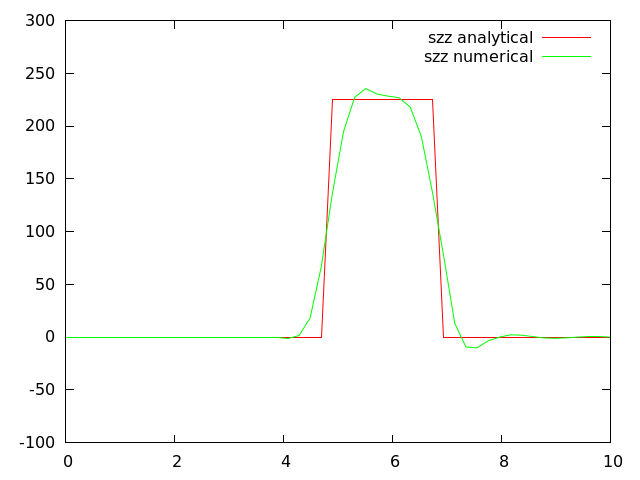
\includegraphics[width=0.75\textwidth]{png/veryfication/0.4/p-wave-along-z15.png}
\caption{15-ый шаг}
\end{subfigure}
\caption{Распространение P-волны вдоль оси $Z$. Показана $\sigma_{zz}$ компонента. Размер тетраэдра -- 0.4, шаг по времени -- 0.000533. }
\label{pic:p_wave_along_z4}
\end{figure}

\begin{figure}[H]
\begin{subfigure}[b]{0.5\textwidth}
\centering
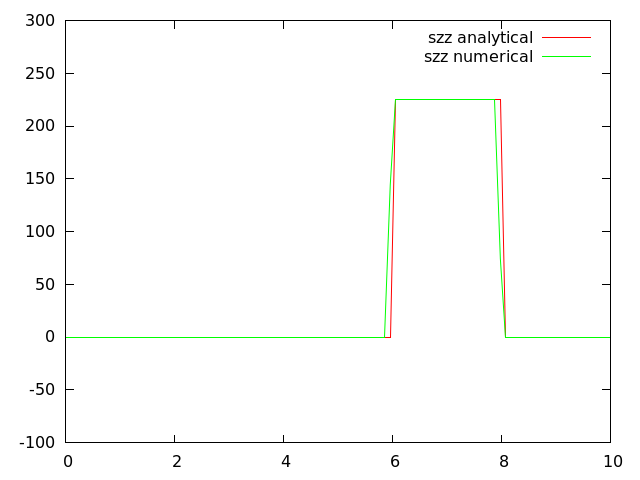
\includegraphics[width=0.75\textwidth]{png/veryfication/0.2/p-wave-along-z0.png}
\caption{Начальное состояние}
\end{subfigure}
\begin{subfigure}[b]{0.5\textwidth}
\centering
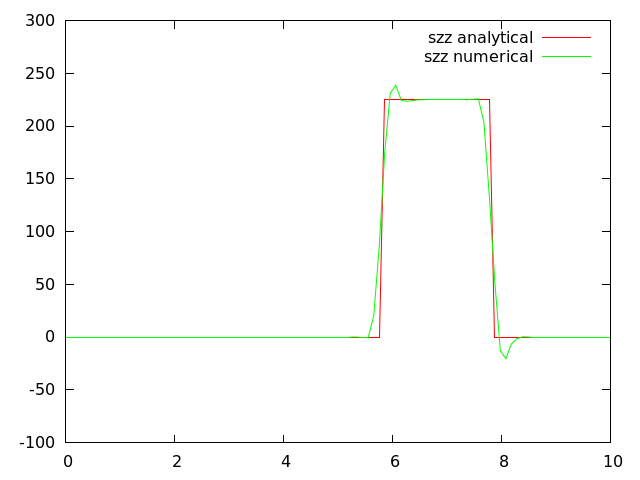
\includegraphics[width=0.75\textwidth]{png/veryfication/0.2/p-wave-along-z5.png}
\caption{5-ый шаг}
\end{subfigure}
\begin{subfigure}[b]{0.5\textwidth}
\centering
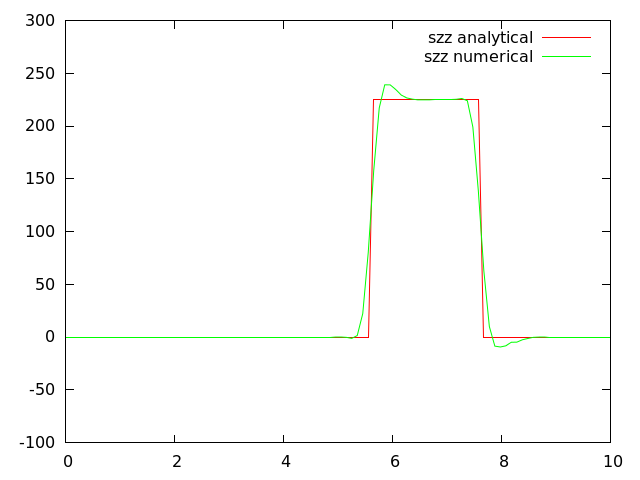
\includegraphics[width=0.75\textwidth]{png/veryfication/0.2/p-wave-along-z10.png}
\caption{10-ый шаг}
\end{subfigure}
\begin{subfigure}[b]{0.5\textwidth}
\centering
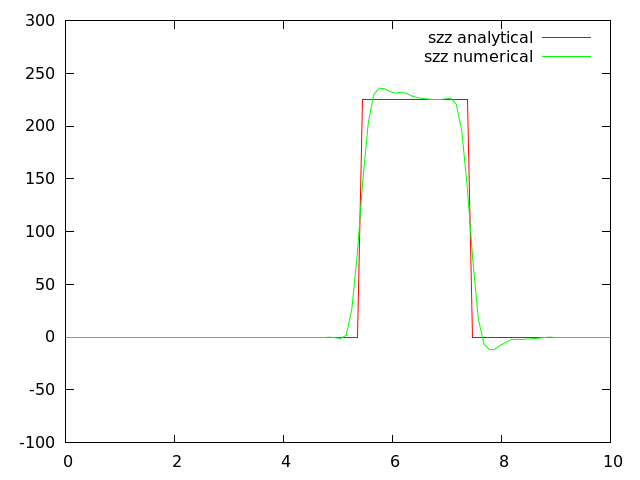
\includegraphics[width=0.75\textwidth]{png/veryfication/0.2/p-wave-along-z15.png}
\caption{15-ый шаг}
\end{subfigure}
\caption{Распространение P-волны вдоль оси $Z$. Показана $\sigma_{zz}$ компонента. Размер тетраэдра -- 0.2, шаг по времени -- 0.000269. }
\label{pic:p_wave_along_z2}
\end{figure}

\begin{figure}[H]
\begin{subfigure}[b]{0.5\textwidth}
\centering
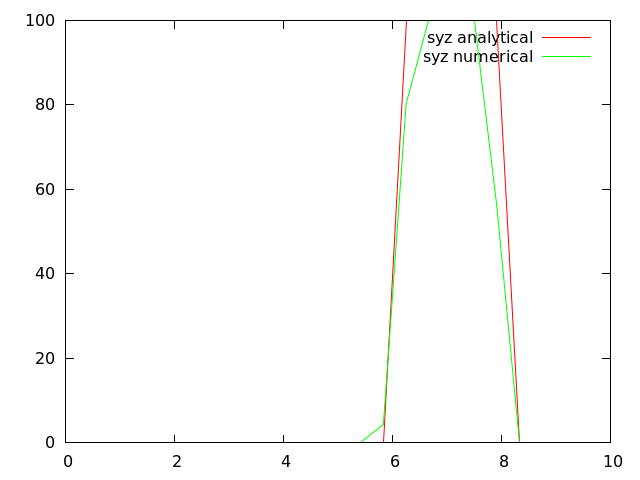
\includegraphics[width=0.75\textwidth]{png/veryfication/0.8/s-wave-along-z0.png}
\caption{Начальное состояние}
\end{subfigure}
\begin{subfigure}[b]{0.5\textwidth}
\centering
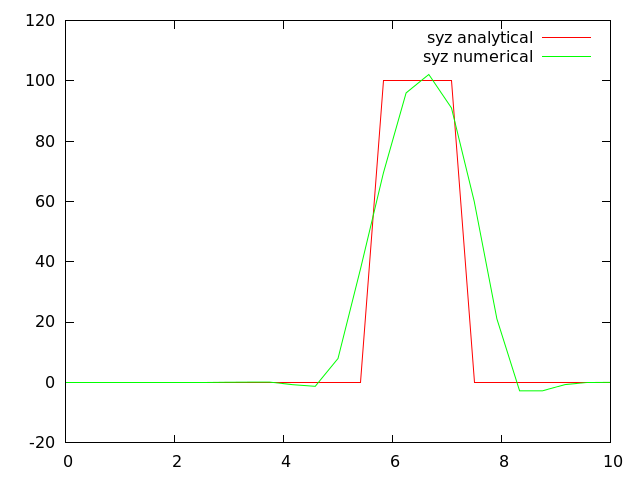
\includegraphics[width=0.75\textwidth]{png/veryfication/0.8/s-wave-along-z5.png}
\caption{5-ый шаг}
\end{subfigure}
\begin{subfigure}[b]{0.5\textwidth}
\centering
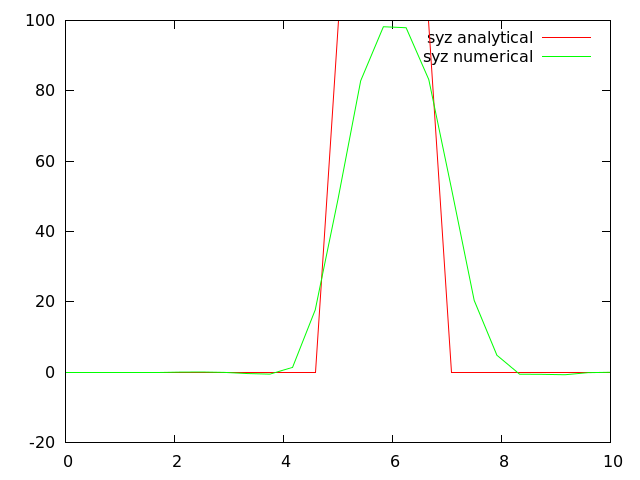
\includegraphics[width=0.75\textwidth]{png/veryfication/0.8/s-wave-along-z10.png}
\caption{10-ый шаг}
\end{subfigure}
\begin{subfigure}[b]{0.5\textwidth}
\centering
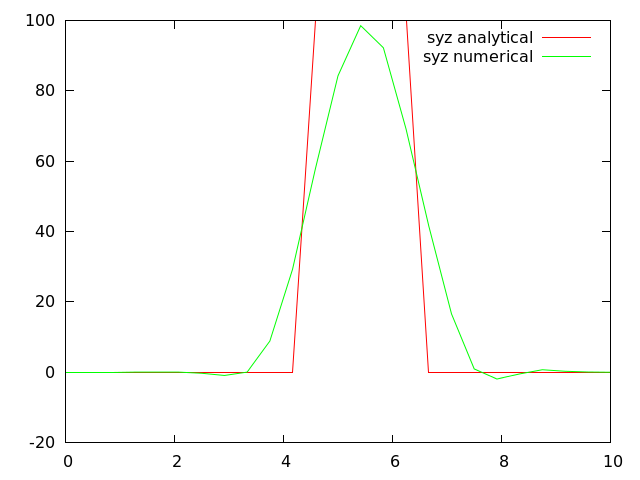
\includegraphics[width=0.75\textwidth]{png/veryfication/0.8/s-wave-along-z15.png}
\caption{15-ый шаг}
\end{subfigure}
\caption{Распространение S-волны вдоль оси $Z$. Показана $\sigma_{yz}$ компонента. Размер тетраэдра -- 0.8, шаг по времени -- 0.001025. }
\label{pic:s_wave_along_z8}
\end{figure}

\begin{figure}[H]
\begin{subfigure}[b]{0.5\textwidth}
\centering
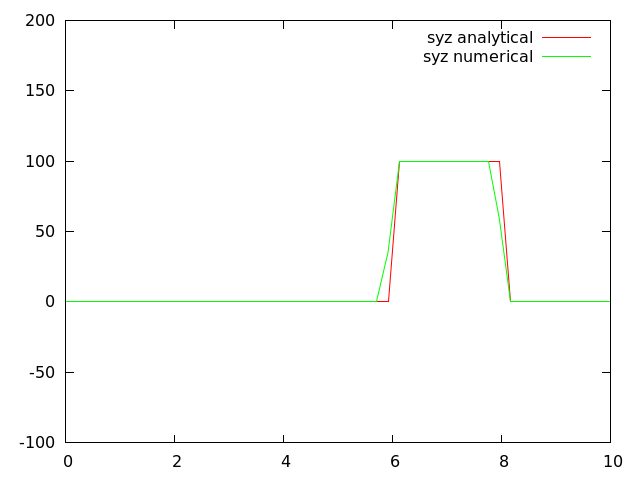
\includegraphics[width=0.75\textwidth]{png/veryfication/0.4/s-wave-along-z0.png}
\caption{Начальное состояние}
\end{subfigure}
\begin{subfigure}[b]{0.5\textwidth}
\centering
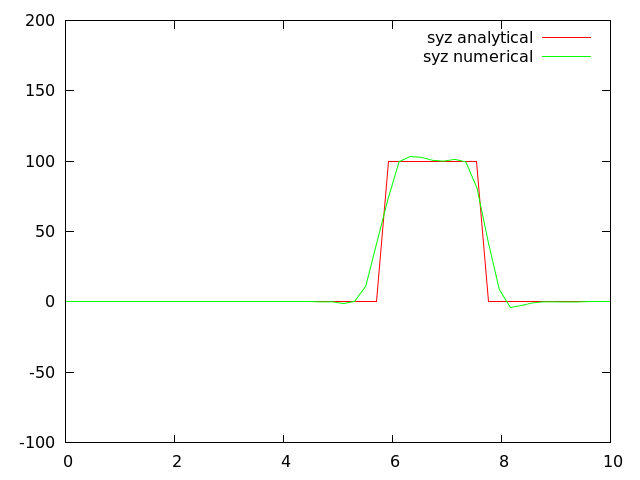
\includegraphics[width=0.75\textwidth]{png/veryfication/0.4/s-wave-along-z5.png}
\caption{5-й шаг}
\end{subfigure}
\begin{subfigure}[b]{0.5\textwidth}
\centering
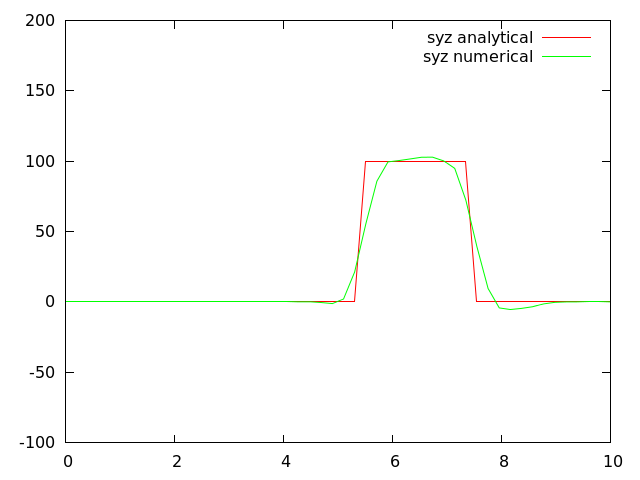
\includegraphics[width=0.75\textwidth]{png/veryfication/0.4/s-wave-along-z10.png}
\caption{10-й шаг}
\end{subfigure}
\begin{subfigure}[b]{0.5\textwidth}
\centering
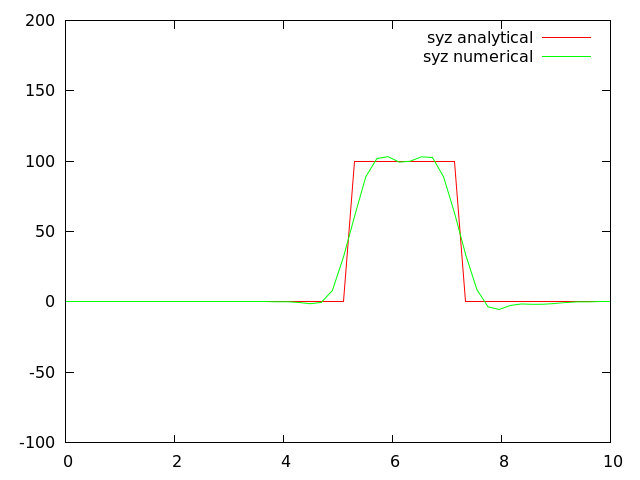
\includegraphics[width=0.75\textwidth]{png/veryfication/0.4/s-wave-along-z15.png}
\caption{15-й шаг}
\end{subfigure}
\caption{Распространение S-волны вдоль оси $Z$. Показана $\sigma_{yz}$ компонента. Размер тетраэдра -- 0.4, шаг по времени -- 0.000533. }
\label{pic:s_wave_along_z4}
\end{figure}

\begin{figure}[H]
\begin{subfigure}[b]{0.5\textwidth}
\centering
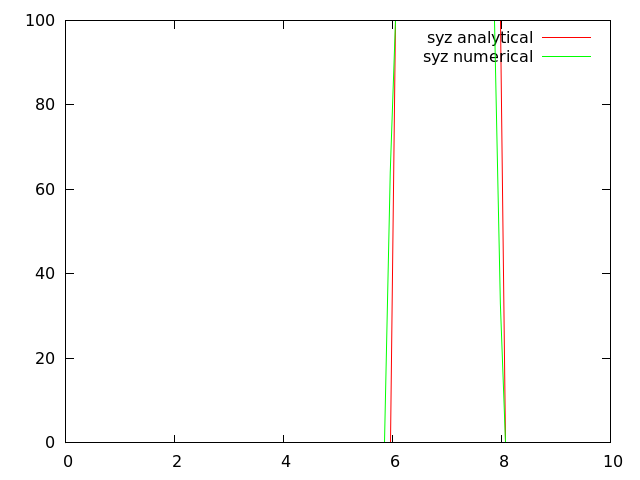
\includegraphics[width=0.75\textwidth]{png/veryfication/0.2/s-wave-along-z0.png}
\caption{Начальное состояние}
\end{subfigure}
\begin{subfigure}[b]{0.5\textwidth}
\centering
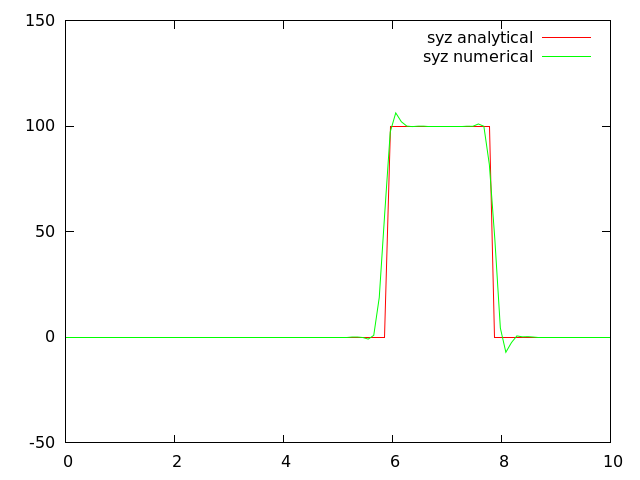
\includegraphics[width=0.75\textwidth]{png/veryfication/0.2/s-wave-along-z5.png}
\caption{5-ый шаг}
\end{subfigure}
\begin{subfigure}[b]{0.5\textwidth}
\centering
\includegraphics[width=0.75\textwidth]{png/veryfication/0.2/s-wave-along-z10.png}
\caption{10-ый шаг}
\end{subfigure}
\begin{subfigure}[b]{0.5\textwidth}
\centering
\includegraphics[width=0.75\textwidth]{png/veryfication/0.2/s-wave-along-z15.png}
\caption{15-ый шаг}
\end{subfigure}
\caption{Распространение S-волны вдоль оси $Z$. Показана $\sigma_{yz}$ компонента. Размер тетраэдра -- 0.2, шаг по времени -- 0.000269. }
\label{pic:s_wave_along_z2}
\end{figure}

	Из рисунков можно сделать вывод, что численные решения распространения P и S волн совпадают с их аналитическими аналогами с точностью до погрешности метода и аналитического приближения.
	Также из рисунков видно, что присутствует сходимость по пространству, однако определить её точное значение по этим данным невозможно, так как полученное значение будет сильно занижено, по сравнению с реальным, в силу грубого аналитического приближения трёхмерной задачи.

\subsection{Расчёт точечного взрыва в однородном теле}

	Был произведён расчёт точечного взрыва в изотропном и ортотропном телах.
	Ниже приведены плоские картинки для сравнения взрыва в изотропной и анизотропной средах.
	
	На Рис. \ref{pic:isotropic-explosion} показаны сферические волны модуля скорости среды в изотропном материале.
	На Рис. \ref{pic:anisotropic-explosion1} представлено то же самое, только в анизотропной среде.
	Вид фронта сферических волн здесь принимает форму эллипса, а также можно наблюдать распространение сдвиговых волн \cite{ogurtsov}, амплитуда которых максимальна на направлении, составляющем 45 градусов с осями.
	Эти волны -- существенное проявление анизотропии материала, в изотропном случае их нет.
	На Рис. \ref{pic:anisotropic-explosion2} изображено отражение волн в анизотропном случае.
	
\begin{figure}[H]
\centerline{\includegraphics[width=0.75\textwidth]{png/dotted_explosion/exp_i_00.png}}
\caption{Точечный взрыв в изотропном теле. Плоский срез. Сферические волны амлитуды скорости.}
\label{pic:isotropic-explosion}
\end{figure}

\begin{figure}[H]
\centerline{\includegraphics[width=0.75\textwidth]{png/dotted_explosion/exp_ai_00.png}}
\caption{Точечный взрыв в анизотропном теле. Плоский срез. Сферические волны амлитуды скорости, а также видны сдвиговые волны рапространяющие под 45 градусов к осям.}
\label{pic:anisotropic-explosion1}
\end{figure}

\begin{figure}[H]
\centerline{\includegraphics[width=0.75\textwidth]{png/dotted_explosion/exp_ai_01.png}}
\caption{Точечный взрыв в анизотропном теле. Плоский срез. Отражение от границ.}
\label{pic:anisotropic-explosion2}
\end{figure}

\subsection{Расчёт двухслойной панели}

	Как уже было сказано, ПКМ -- многослойные анизотропные материалы, каждый субпакет которых включает в себя несколько слоев ортотропного материала, по-разному ориентированных вокруг оси укладки.
	Здесь мы рассмотрим расчёты динамического нагружения двухслойки, как некоторой минимальльной компоненты субпакета ПКМ.

	Под двухслойкой здесь мы понимаем два слоя трансверсально-изотропного материала, выделенные направления которых лежат в плоскости слоёв и составляют прямой угол друг с другом.
	Для начала используем тот же модельный материал, что мы использовали ранее:
\begin{align}
\label{model_mat}
\left( \begin{array}{cccccccccccc}
90000 & 70000 & 17500 & 0 & 0 & 0 \\ 
70000 & 90000 & 17500 & 0 & 0 & 0 \\ 
17500 & 17500 & 22500 & 0 & 0 & 0 \\ 
0 & 0 & 0 & 10000 & 0 & 0 \\ 
0 & 0 & 0 & 0 & 10000 & 0 \\ 
0 & 0 & 0 & 0 & 0 & 10000
\end{array} \right),
\end{align}	
\begin{equation}
	\rho = 1.
\end{equation}
	
	На рисунках снизу показано разделение на слои заданной области и вид начальной нагрузки -- удар прямоугольного профиля по поверхности верхнего слоя.	
\begin{figure}[H]
\begin{subfigure}[b]{0.5\textwidth}
\centering
\includegraphics[width=0.9\textwidth]{png/two-layers/view.png}
\caption{Разделение на слои.}
\end{subfigure}
\begin{subfigure}[b]{0.5\textwidth}
\centering
\includegraphics[width=0.9\textwidth]{png/two-layers/initial_view.png}
\caption{Вид начальной нагрузки.}
\end{subfigure}
\caption{Вид расчётной области.}
\label{pic:two_layers_view}
\end{figure}

	Ниже представлены изображения распространения волн в срезе четверти слоя.
	Тут отлично прослеживается анизотропия распростванения возмущений в слоях.
	Кроме того на последнем рисунке можно заметить как волна распространявшаяся медленно вдоль оси $Y$, войдя во второй слой ускорилась.
\begin{figure}[H]
\begin{subfigure}[b]{0.5\textwidth}
\centering
\includegraphics[width=1.0\textwidth]{png/two-layers/clip2_0.png}
\caption{Начальное состояние}
\end{subfigure}
\begin{subfigure}[b]{0.5\textwidth}
\centering
\includegraphics[width=1.0\textwidth]{png/two-layers/clip2_10.png}
\caption{10-ый шаг}
\end{subfigure}
\begin{subfigure}[b]{0.5\textwidth}
\centering
\includegraphics[width=1.0\textwidth]{png/two-layers/clip2_20.png}
\caption{20-ый шаг}
\end{subfigure}
\begin{subfigure}[b]{0.5\textwidth}
\centering
\includegraphics[width=1.0\textwidth]{png/two-layers/clip2_30.png}
\caption{30-ый шаг}
\end{subfigure}
\begin{subfigure}[b]{0.5\textwidth}
\centering
\includegraphics[width=1.0\textwidth]{png/two-layers/clip2_40.png}
\caption{40-ой шаг}
\end{subfigure}
\begin{subfigure}[b]{0.5\textwidth}
\centering
\includegraphics[width=1.0\textwidth]{png/two-layers/clip2_50.png}
\caption{50-й шаг}
\end{subfigure}
\caption{Распространение деформаций в двухслойке. Двойной срез. Цветом отмечены волны амплитуды скорости.}
\label{pic:two_layers_clip2}
\end{figure}

\begin{figure}[H]
\begin{subfigure}[b]{0.5\textwidth}
\centering
\includegraphics[width=1.0\textwidth]{png/two-layers/slice_20.png}
\caption{20-ый шаг}
\end{subfigure}
\begin{subfigure}[b]{0.5\textwidth}
\centering
\includegraphics[width=1.0\textwidth]{png/two-layers/slice_30.png}
\caption{30-ый шаг}
\end{subfigure}
\begin{subfigure}[b]{0.5\textwidth}
\centering
\includegraphics[width=1.0\textwidth]{png/two-layers/slice_40.png}
\caption{40-ой шаг}
\end{subfigure}
\begin{subfigure}[b]{0.5\textwidth}
\centering
\includegraphics[width=1.0\textwidth]{png/two-layers/slice_50.png}
\caption{50-ый шаг}
\end{subfigure}
\caption{Распространение деформаций в двухслойке. Вид сверху. Цветом отмечены волны амплитуды скорости.}
\label{pic:two_layers_top}
\end{figure}

	Сильно выраженными анизотропными свойствами обладает графит.
	Это связано с тем, что некоторые компоненты матрицы упругих постоянных отличаются у него на несколько порядков:
\begin{align}
\label{graphite_mat}
\left( \begin{array}{cccccccccccc}
1060000 & 180000 & 15000 & 0 & 0 & 0 \\ 
180000 & 1060000 & 15000 & 0 & 0 & 0 \\ 
15000 & 17500 & 37000 & 0 & 0 & 0 \\ 
0 & 0 & 0 & 200 & 0 & 0 \\ 
0 & 0 & 0 & 0 & 200 & 0 \\ 
0 & 0 & 0 & 0 & 0 & 440000
\end{array} \right),
\end{align}	
\begin{equation}
	\rho = 2.1.
\end{equation}
	Здесь упругие постоянные указаны в МПа, а плотность в граммах на кубический сантиметр.
	
	Рассмотрим ту же постановку задачи с двухслойкой, только теперь в качестве материала возьмём графит.
	Вид рассмотриваемой области и начальное воздействие аналогичны Рис. \ref{pic:two_layers_view}.
	
\begin{figure}[H]
\begin{subfigure}[b]{0.5\textwidth}
\centering
\includegraphics[width=1.0\textwidth]{png/two-graphite-layers/2clip0.png}
\caption{Начальное состояние}
\end{subfigure}
\begin{subfigure}[b]{0.5\textwidth}
\centering
\includegraphics[width=1.0\textwidth]{png/two-graphite-layers/2clip10.png}
\caption{10-ый шаг}
\end{subfigure}
\begin{subfigure}[b]{0.5\textwidth}
\centering
\includegraphics[width=1.0\textwidth]{png/two-graphite-layers/2clip20.png}
\caption{20-ый шаг}
\end{subfigure}
\begin{subfigure}[b]{0.5\textwidth}
\centering
\includegraphics[width=1.0\textwidth]{png/two-graphite-layers/2clip30.png}
\caption{30-ый шаг}
\end{subfigure}
\begin{subfigure}[b]{0.5\textwidth}
\centering
\includegraphics[width=1.0\textwidth]{png/two-graphite-layers/2clip40.png}
\caption{40-ой шаг}
\end{subfigure}
\begin{subfigure}[b]{0.5\textwidth}
\centering
\includegraphics[width=1.0\textwidth]{png/two-graphite-layers/2clip50.png}
\caption{50-ый шаг}
\end{subfigure}
\begin{subfigure}[b]{0.5\textwidth}
\centering
\includegraphics[width=1.0\textwidth]{png/two-graphite-layers/2clip60.png}
\caption{60-ый шаг}
\end{subfigure}
\caption{Распространение деформаций в двухслойке из графита. Двойной срез. Цветом отмечены волны амплитуды скорости.}
\label{pic:two_graphite_clip2}
\end{figure}

	Рисунки очень показательны.
	Во-первых, распространения волн вдоль оси $Z$ практически нет, так как компонента в \eqref{graphite_mat}, отвечающая за скорость распространения волны вдоль этой оси на несколько порядков ниже своих аналогов для остальных осей.
	Во-вторых, волна, пришедшая во второй слой начинает заметно распространяться вдоль оси $Z$, так как нижний слой повернут на величину прямого улга, по сравнению с верхним.
	В этом плане также показательны следующие изображения среза плоскости $XZ$.
	
\begin{figure}[H]
\begin{subfigure}[b]{0.5\textwidth}
\centering
\includegraphics[width=1.0\textwidth]{png/two-graphite-layers/xz5.png}
\caption{5-ый шаг}
\end{subfigure}
\begin{subfigure}[b]{0.5\textwidth}
\centering
\includegraphics[width=1.0\textwidth]{png/two-graphite-layers/xz15.png}
\caption{15-ый шаг}
\end{subfigure}
\begin{subfigure}[b]{0.5\textwidth}
\centering
\includegraphics[width=1.0\textwidth]{png/two-graphite-layers/xz30.png}
\caption{30-ый шаг}
\end{subfigure}
\begin{subfigure}[b]{0.5\textwidth}
\centering
\includegraphics[width=1.0\textwidth]{png/two-graphite-layers/xz40.png}
\caption{40-ой шаг}
\end{subfigure}
\begin{subfigure}[b]{0.5\textwidth}
\centering
\includegraphics[width=1.0\textwidth]{png/two-graphite-layers/xz50.png}
\caption{50-ый шаг}
\end{subfigure}
\begin{subfigure}[b]{0.5\textwidth}
\centering
\includegraphics[width=1.0\textwidth]{png/two-graphite-layers/xz58.png}
\caption{58-ый шаг}
\end{subfigure}
\caption{Распространение деформаций в двухслойке из графита. Срез плоскости $XZ$. Цветом отмечены волны амплитуды скорости.}
\label{pic:two_graphite_xz}
\end{figure}
	
	Также стоит взглянуть на картину распространения волн в срезе перпендикулярном начальному возмущению в обоих слоях.
	Если в первом слое в срезе волны распространяются лишь вдоль оси $Y$, то во втором эта ситуация меняется, и полученная картина начинает растягиваться вдоль оси $Z$.
	
\begin{figure}[H]
\begin{subfigure}[b]{0.5\textwidth}
\centering
\includegraphics[width=1.0\textwidth]{png/two-graphite-layers/slice_15.png}
\caption{15-ый шаг}
\end{subfigure}
\begin{subfigure}[b]{0.5\textwidth}
\centering
\includegraphics[width=1.0\textwidth]{png/two-graphite-layers/slice_30.png}
\caption{30-ый шаг}
\end{subfigure}
\begin{subfigure}[b]{0.5\textwidth}
\centering
\includegraphics[width=1.0\textwidth]{png/two-graphite-layers/slice_40.png}
\caption{40-ой шаг}
\end{subfigure}
\begin{subfigure}[b]{0.5\textwidth}
\centering
\includegraphics[width=1.0\textwidth]{png/two-graphite-layers/slice_50.png}
\caption{50-ый шаг}
\end{subfigure}
\caption{Распространение деформаций в двухслойке из графита. Срез в первом слое, ортогонально начальной нагрузке. Цветом отмечены волны амплитуды скорости.}
\label{pic:two_graphite_slice1}
\end{figure}

\begin{figure}[H]
\begin{subfigure}[b]{0.5\textwidth}
\centering
\includegraphics[width=1.0\textwidth]{png/two-graphite-layers/slice2_45.png}
\caption{45-ый шаг}
\end{subfigure}
\begin{subfigure}[b]{0.5\textwidth}
\centering
\includegraphics[width=1.0\textwidth]{png/two-graphite-layers/slice2_50.png}
\caption{50-ый шаг}
\end{subfigure}
\begin{subfigure}[b]{0.5\textwidth}
\centering
\includegraphics[width=1.0\textwidth]{png/two-graphite-layers/slice2_55.png}
\caption{55-ый шаг}
\end{subfigure}
\begin{subfigure}[b]{0.5\textwidth}
\centering
\includegraphics[width=1.0\textwidth]{png/two-graphite-layers/slice2_60.png}
\caption{60-ый шаг}
\end{subfigure}
\caption{Распространение деформаций в двухслойке из графита. Срез во втором слое, ортогонально начальной нагрузке. Цветом отмечены волны амплитуды скорости.}
\label{pic:two_graphite_slice2}
\end{figure}

\subsection{Расслоение}
	
	Многие современные исследования динамической нагрузки ПКМ используют различные осреднённые модели композитного материала.
	Вместо представления о субпакете композита как о слоистой анизотропной структуре вводятся эффективные осреднённые прочностные характеристики изучаемого материала \cite{bahvalov}.
	Этот подход во многом оправдан: с одной стороны, строгие математические постоения осреднённых моделей ПКМ позволили более глубого понять процессы, происходящие в них, с другой, исследование осреднённых структур в вычислительном плане более дешёвая задача, по сравнению с расчётом, явно учитывающим всю структуру субпакета композитной панели.
	Тем не менее осреднение слоистых структур не позволяет наблюдать эффекты расслоения, которые в свою очередь могут серьезным образом сказаться на прочностных характеристиках ПКМ.
	
	Эффекты расслоения слоистого материала, в смысле разрушения контакта между слоями, а также разрушения контакта между матрицей и армирующими волокнами ПКМ относятся к понятию \textit{адгезионной прочности} материала.
	Здесь мы рассмотрим расчёты разрушения контакта между двумя скрещенными слоями модельного ортотропного материала.
	
\subsubsection{Разрушения контакта}

	Разрушение контакта двух слоёв моделируется следующим образом.
	Каждый контактирующий узел сетки может находится в двух состояниях: разрушенном или неразрушенном.
	Для разрушенного узла производится расчёт по \textit{схеме с чистым скольжением} (или с некоторым трением) на контакте. 
	Такой узел не может перейти в неразрушенное состояние.
	
	Для неразрушенного узла сетки вычисления производятся по следующему алгоритму:
	
\begin{enumerate}
	\item Производится расчёт \textit{по схеме полного слипания}:
	\begin{equation}
		v_n = \widetilde{v_n}, \quad v_{\tau0} = \widetilde{v_{\tau0}}, \quad v_{\tau1} = \widetilde{v_{\tau1}},
	\end{equation}
		где $v$ и $\widetilde{v}$ обозначают скорости контактных узлов первого и второго слоёв соответственно.
	\item Вычисляется нормальная сила действующая на узлы и подставляется в критерий разрушения контакта:
	\begin{align}
		\vec{f} = \sigma \vec{n}, \\
		|\vec{f}| \geq f_0,
	\end{align}
		где $f_0$ -- адгезионная прочность.
	\item В случае выполнения критерия расчёт считается некоректным, узел переводится в класс разрушенных, и выполняется расчёт для разрушенного узла. В противном случае расчёт признаётся корректным.
\end{enumerate}
	
\subsubsection{Расчёты}

	Ниже представлены расчёты разрушения контакта между двумя скрещенными слоями модельного ортотропного материала с параметрами: 
\begin{align}
\label{delamination_model_mat}
\left( \begin{array}{cccccccccccc}
180000 & 70000 & 70000 & 0 & 0 & 0 \\ 
70000 & 90000 & 70000 & 0 & 0 & 0 \\ 
70000 & 70000 & 90000 & 0 & 0 & 0 \\ 
0 & 0 & 0 & 10000 & 0 & 0 \\ 
0 & 0 & 0 & 0 & 20000 & 0 \\ 
0 & 0 & 0 & 0 & 0 & 20000
\end{array} \right),
\end{align}	
\begin{align}
	\rho = 1,\\
	f_0 = 100.
\end{align}
	
	Начальная постановка задачи выглядин следующим образом:
\begin{figure}[H]
\centerline{\includegraphics[width=0.6\textwidth]{png/delamination/mat_view.png}}
\caption{Удар шарика по поверхности двухслойной конструкции. Разделение на слои.}
\label{pic:delamination_view}
\end{figure}

\begin{figure}[H]
\begin{subfigure}[b]{0.5\textwidth}
\centering
\includegraphics[width=1.0\textwidth]{png/delamination/velocity/0.png}
\caption{Начальное состояние}
\end{subfigure}
\begin{subfigure}[b]{0.5\textwidth}
\centering
\includegraphics[width=1.0\textwidth]{png/delamination/velocity/50.png}
\caption{50-ый шаг}
\end{subfigure}
\begin{subfigure}[b]{0.5\textwidth}
\centering
\includegraphics[width=1.0\textwidth]{png/delamination/velocity/100.png}
\caption{100-ый шаг}
\end{subfigure}
\begin{subfigure}[b]{0.5\textwidth}
\centering
\includegraphics[width=1.0\textwidth]{png/delamination/velocity/120.png}
\caption{120-ый шаг}
\end{subfigure}
\begin{subfigure}[b]{0.5\textwidth}
\centering
\includegraphics[width=1.0\textwidth]{png/delamination/velocity/150.png}
\caption{150-ый шаг}
\end{subfigure}
\begin{subfigure}[b]{0.5\textwidth}
\centering
\includegraphics[width=1.0\textwidth]{png/delamination/velocity/200.png}
\caption{200-ый шаг}
\end{subfigure}
\caption{Распространение волн амплитуды скорости вблизи контакта. Разрез первого слоя.}
\label{pic:delamination_velocity}
\end{figure}

	Уже на этих изображениях виден контраст модулей скорости в приконтактной области по разные стороны он границы (100-ый, 120-ый шаги).
	
	Ниже представлены изображения с областями разрушенного контакта в нижнем слое.
	
\begin{figure}[H]
\begin{subfigure}[b]{0.5\textwidth}
\centering
\includegraphics[width=1.0\textwidth]{png/delamination/single_clip/0.png}
\caption{Начальное состояние}
\end{subfigure}
\begin{subfigure}[b]{0.5\textwidth}
\centering
\includegraphics[width=1.0\textwidth]{png/delamination/single_clip/20.png}
\caption{20-ый шаг}
\end{subfigure}
\begin{subfigure}[b]{0.5\textwidth}
\centering
\includegraphics[width=1.0\textwidth]{png/delamination/single_clip/70.png}
\caption{70-ый шаг}
\end{subfigure}
\begin{subfigure}[b]{0.5\textwidth}
\centering
\includegraphics[width=1.0\textwidth]{png/delamination/single_clip/90.png}
\caption{90-ый шаг}
\end{subfigure}
\begin{subfigure}[b]{0.5\textwidth}
\centering
\includegraphics[width=1.0\textwidth]{png/delamination/single_clip/100.png}
\caption{100-ый шаг}
\end{subfigure}
\begin{subfigure}[b]{0.5\textwidth}
\centering
\includegraphics[width=1.0\textwidth]{png/delamination/single_clip/120.png}
\caption{120-ый шаг}
\end{subfigure}
\begin{subfigure}[b]{0.5\textwidth}
\centering
\includegraphics[width=1.0\textwidth]{png/delamination/single_clip/150.png}
\caption{150-ый шаг}
\end{subfigure}
\begin{subfigure}[b]{0.5\textwidth}
\centering
\includegraphics[width=1.0\textwidth]{png/delamination/single_clip/200.png}
\caption{200-й шаг}
\end{subfigure}
\caption{Распространение волн амплитуды скорости в первом слое. Области рарушенного контакта во втором (нижнем) слое. Разрез первого слоя.}
\label{pic:delamination_single_clip}
\end{figure}

\begin{figure}[H]
\begin{subfigure}[b]{0.5\textwidth}
\centering
\includegraphics[width=1.0\textwidth]{png/delamination/double_clip/0.png}
\caption{Начальное состояние}
\end{subfigure}
\begin{subfigure}[b]{0.5\textwidth}
\centering
\includegraphics[width=1.0\textwidth]{png/delamination/double_clip/25.png}
\caption{25-ый шаг}
\end{subfigure}
\begin{subfigure}[b]{0.5\textwidth}
\centering
\includegraphics[width=1.0\textwidth]{png/delamination/double_clip/80.png}
\caption{80-ый шаг}
\end{subfigure}
\begin{subfigure}[b]{0.5\textwidth}
\centering
\includegraphics[width=1.0\textwidth]{png/delamination/double_clip/90.png}
\caption{90-ый шаг}
\end{subfigure}
\begin{subfigure}[b]{0.5\textwidth}
\centering
\includegraphics[width=1.0\textwidth]{png/delamination/double_clip/100.png}
\caption{100-ый шаг}
\end{subfigure}
\begin{subfigure}[b]{0.5\textwidth}
\centering
\includegraphics[width=1.0\textwidth]{png/delamination/double_clip/150.png}
\caption{150-ый шаг}
\end{subfigure}
\begin{subfigure}[b]{0.5\textwidth}
\centering
\includegraphics[width=1.0\textwidth]{png/delamination/double_clip/200.png}
\caption{200-ый шаг}
\end{subfigure}
\begin{subfigure}[b]{0.5\textwidth}
\centering
\includegraphics[width=1.0\textwidth]{png/delamination/double_clip/250.png}
\caption{250-й шаг}
\end{subfigure}
\caption{Распространение волн амплитуды скорости в первом слое. Области рарушенного контакта во втором (нижнем) слое. Двойной разрез первого слоя, вид сверху.}
\label{pic:delamination_double_clip}
\end{figure}

	На этих изображениях чётко виден процесс расслоения.
	Медленная волна, распространяющаяся вдоль оси $Y$, достигнув границы слоёв на некотором расстоянии от центра, на чинает распространяться с большей скоростью.

\clearpage
\newpage
\section*{Заключение}
\addcontentsline{toc}{section}{Заключение}
\setcounter{subsection}{0}

	Можно выделить основные результаты данной работы:	
\begin{enumerate}
	\item На начальном этапе было проведено изучение литературы по механике сплошных сред, численным методам расчёта упругих деформаций в твёрдых изотропных и анизотроных материалах, подробное изучение сеточно-характерестического метода.
			Далее были изучены особенности механики ПКМ и численного моделирования слоистых структур. Был подробно рассмотрен ряд научных статей по моделированию динамических задач МДТТ.
	\item Написана модификация существующего пакета расчёта динамических задач МДТТ сеточно-характеристическим методом позволяющая производить расчёты анизотропных тел.
	\item Поставлен и успешно проведён ряд тестовых задач распространения P и S волн в анизотропном теле для проверки написанной модификации.
	\item Произведены расчёты точечного взрыва в однородном изотропном и анизотропном телах, демонстрирующие наличие дополнительных сдвиговых волн в анизотропном случае (по сравнению с изотропным). Эти волны были ранее предсказаны в \cite{ogurtsov}.
	\item Выполнен ряд расчётов динамического нагружения двухслойной конструкции, иллюстрирующих изменение формы фронтов волн при переходе между слоями.
	\item Получен эффект расслоения контакта двух анизотропных слоёв при динамическом нагружении. Форма разрушенной области совпадает результатами других численных и экспериментальных рассмотрений \cite{serge}.
\end{enumerate}

	Ряд основных результов моделирования волн упругих деформаций в анизотропных телах был представлен в работе:
	\begin{itemize}
		\item Петров И.Б., Фаворская А.В., Васюков А.В., Ермаков А.С., Беклемышева К.А., Казаков А.О., Новиков А.В. <<О численном моделировании волновых процессов в анизотропных средах>>. // Журнал <<Доклады Академии Наук>>. - 2014.
	\end{itemize}

\clearpage
\newpage
\begin{thebibliography}{99}
\addcontentsline{toc}{section}{Список использованных источников}

% Численные методы
\bibitem{petrov_book}Петров И.Б., Лобанов А.И. Лекции по вычислительной математике: Учебное пособие -- М.: Интернет-Университет Информационных Технологий; БИНОМ.Лаборатория знаний, 2013.-523 с.: ил., табл. -- (Серия <<Основы информационных технологий>>)
\bibitem{magomedov}Магомедов К.М., Холодов А.С. Сеточно-характеристические численные методы. -- М.: Наука, 1988, 288 с.
\bibitem{jp}Сиратори М., Миёси Т., Мацусита Х. Вычислительная механика разрушения. // М.: Мир, 1986. -- 334 с.
\bibitem{kukudzhanov_main}Кукуджанов В.Н. Вычислительная механика сплошных сред. -- М.: Издательство физико-математической литематуры, 2008. -- 320 с.
\bibitem{uilkins}Уилкинс М.Л. Расчёт упругопластических течений. В кн.: Вычислительные методы в гидродинамике. -- М.: Мир, 1967. С.212-163.
\bibitem{belocerkovsky}Белоцерковский О.М. Численное моделирование в механике сплошных сред. — М.: Физико-математическая литература. 1994, 442 с.
\bibitem{fedorenko}Федоренко Р.П. Введение в вычислительную физику. М.:Изд-во Моск. физ. -техн. ин-та, 1994, 528 с.
\bibitem{kukudzhanov1}Кукуджанов В.Н. Распространение упругопластических волн в стержне с учётом влияния скорости деформации. -- М.: ВЦ АН СССР, 1967. С.48.
\bibitem{kukudzhanov2}Кукуджанов В.Н. Численное решение неодномерных задач распространения волн напряжений в твёрдых телах//Сообщение по прикладной математике ВЦ. 1976. Вып. 6. С.67.
\bibitem{bahvalov}Бахвалов Н.С., Панасенко Г.П. Осреднение процессов в периодических средах — математические задачи механики композиционных материалов. 1984

% Физика 
\bibitem{novatsky}Новацкий В. К. Теория упругости. — М. : Мир, 1975, c. 105-107.
\bibitem{sedov}Седов Л. И. Механика сплошной среды. Том 1. — М. : Наука, 1970, с. 143.
\bibitem{rabotnov}Работнов Ю.Н. Механика деформируемого твёрдого тела. — М.: Наука, 1988. — 712 с.
\bibitem{landau_lifshits}Ландау Л.Д., Лифшиц Е.М. Теория упругости. М.: Наука, Главная редакция физико-математической литературы, 1965.
\bibitem{ilyushin}Ильюшин А.А. Пластичность. М.: ОГИЗ, Государственное издательство технико-теоретической литературы, 1948
\bibitem{lehnitsky}Лехницкий С.Г. Теория упругости анизотропного тела. Изд. 2-е, Главная редакция физико-математической литературы издательства <<Наука>>, М., 1977, 416 стр.

% Композиты vs. Анизотропия
\bibitem{simamura}Под. ред. С.Симамуры. Углеродные волокна: Пер. с япон. -- М.:Мир, 1987 - 304 с., ил.
\bibitem{pobedrya}Победря Б.Е. Механика композиционных материалов. -- М.:Изд-во Моск. ун-та, 1984. -- 336 с.
\bibitem{bazhenov}Баженов С.Л., Берлин А.А., Кульков А.А., Ошмян В.Г. Полимерные композиционные материалы. - Долгопрудный: Издательский дом Интеллект, 2010, 352 с.
\bibitem{resler}Реслер И., Хардерс Х., Бекер М. Механическое поведение конструкционных материалов. Пер. с нем. Учебное пособие -- Долгопрудный Издательский Дом <<Интеллект>>, 2011. -- 504 с.
\bibitem{serge}Serge Abrate. Impact on composite structures. Cambridge University Press, 2005. 

% Математика
\bibitem{rozhdestvenskiy}Рождественский Б.Л., Яненко Н.Н. Системы квазилинейных уравнений и их приложения к газовой динамике. -- М.: Наука, 1968.--592 с.
\bibitem{kulikovskiy}Куликовский A.Г., Погорелов Н.В., Семенов А.Ю. Математические вопросы численного решения гиперболических систем уравнений.--М.:ФИЗМАТЛИТ, 2001.--608 с.
\bibitem{ogurtsov}Огурцов К.И., Пахоменко Л.С. Анализ упругих волн, возбуждаемых сосредоточенными источниками в анизотропных средах.Распространение упругих и упруго-пластических волн (Материалы 3-го Всесоюзн. симпозиума. Сборник статей.) Т., <<Фан>>, 1969. 448 с.

% Работы Кафедры Информатики
\bibitem{favorskaya}Фаворская А. В. Постановка задачи численного моделирования динамических про-цессов в сплошной линейно-упругой среде с анизотропией сеточно-характеристическим методом // Труды 54-й научной конференции МФТИ: Пробле-мы фундаментальных и прикладных наук в современном информационном общест-ве. — 2011. — Т. 2. — С. 55 – 56.
\bibitem{g}Иванов В.Д., Кондауров В.Н., Холодов А.С. Расчет динамического деформирования и разрушения упругопластических тел сеточно-характеристическими методами. // Математическое моделирование, 2003, Т. 15, № 10.
\bibitem{petrov_tormasov_holodov}Петров  И.Б., Тормасов А.Г., Холодов А.С. О численном изучении нестационарных процессов в деформируемых средах многослойной структуры // Механика твердого тела – 1989, N 4, с. 89-95.
\bibitem{ivanov_kondaurov_petrov_holodov} Иванов В.Д., Кондауров В.И., Петров И.Б., Холодов А.С. Расчет динамического деформирования и разрушения упругопластических тел сеточно-характеристическими методами – Матем. Моделирование № 2:11, 1990, С. 10 – 29
\bibitem{petrov}Петров И.Б. Волновые и откольные явления в слоистых оболочках конечной толщины // Механика твердого тела – 1986, N 4, с. 118-124.
\bibitem{a4} Васюков А.В., Петров И.Б. О разработке параллельной версии сеточно-характеристического метода для трехмерных уравнений механики деформируемого твердого тела. // Сборник научных трудов <<Модели и методы обработки информации>>. М.: МФТИ, 2009. С. 13--17.
\bibitem{a6} Васюков А.В., Петров И.Б., Черников Д.В. О сеточно"=характеристическом численном методе на неструктурированных сетках для задач механики деформируемого твердого тела в случае трех пространственных переменных. // Сборник научных трудов <<Информационные технологии: модели и методы>>. М.: МФТИ, 2010. С. 52--57.
\bibitem{chelnokov}Челноков Ф.Б. Численное моделирование деформационных процессов в средах со сложной структурой: Дисс. ... канд. физ.-мат. наук – М., 2005

\end{thebibliography}
	

\end{document}
